\documentclass[11pt,a4paper]{article}
\usepackage[utf8]{inputenc}
\usepackage[T1]{fontenc}
\usepackage[brazilian]{babel}
\usepackage[margin=2.3cm]{geometry}
\usepackage{graphicx}
\usepackage{booktabs}
\usepackage{array}
\usepackage{xcolor}
\usepackage{hyperref}
\usepackage{caption}
\usepackage{amsmath}
\usepackage{longtable}
\usepackage{float}
\usepackage{enumitem}
\usepackage{multirow}

\hypersetup{
  colorlinks=true,
  linkcolor=blue!50!black,
  urlcolor=blue!50!black,
  citecolor=blue!50!black
}

\title{Redução de Falso Alerta no Candidato EXP7 Item 1+2\\
\large Do diagnóstico por episódios às três correções que cortaram\\
o falso alerta em $\sim$82\% sem perder nenhuma detecção real}
\author{Pipeline \texttt{cnn1d\_ae} / AutoML --- projeto \texttt{TesteMLCab}}
\date{Agosto de 2026}

\begin{document}
\maketitle

\begin{abstract}
Partindo do candidato de referência EXP7 item 1+2 (\texttt{ocsvm},
multiescala + textura --- 92,5\% de hit\_rate, 1,94\% de falso alerta),
este relatório documenta como investigamos e reduzimos o falso alerta em
$\sim$82\% (para 0,35\%) \textbf{sem perder nenhuma das 32 detecções
reais}. O método: fragmentar a série de anomalias em episódios contínuos,
cruzar cada um com os dados brutos (temperatura, vibração) e com o
catálogo completo de 47 tags de alarme, em vez de confiar só na métrica
agregada. Isso revelou que o falso alerta não é ruído difuso: 65,3\% dele
vem de um único desligamento real de 3,5 dias que a máscara operacional
não reconhecia (\texttt{RUNNING\_A} ficava preso em $\sim$1 enquanto a
temperatura caía a nível ambiente), e mais 25\% vem de rampas de carga
legítimas (variação real de dezenas de graus/hora, sem alarme, sem
falha). Três correções cirúrgicas, todas na camada de pós-processamento
(nenhuma toca no modelo de anomalia em si), resolveram a maior parte
disso: um segundo critério de ``desligado'' baseado no piso físico do
próprio sensor-alvo; um portão de rampa (já existente no pipeline
CNN1D-AE, mas nunca portado para o AutoML) ajustado por simulação
offline até o ponto de custo zero; e um portão de volatilidade novo, que
só existe porque a primeira tentativa (reaproveitar o portão de rampa
para a vibração) não funcionou e a investigação de por que não funcionou
apontou o mecanismo certo. Documentamos também um caminho testado e
descartado --- aumentar o debounce --- com a evidência de por que não
funciona.
\end{abstract}

\tableofcontents

% =====================================================================
\section{Ponto de partida}
% =====================================================================

O candidato de referência da série EXP5--EXP9 é o \texttt{ocsvm}
(percentil 99,9, debounce=1) sobre o grupo \texttt{TC382\_T5\_vibra\-cao\_mancais\_multiescala}
(\texttt{TC382\_03\_A} + \texttt{T5\_AVG\_A} + 10 canais de vibração de
mancal, com features multi-escala e de textura --- EXP7 itens 1+2).
Avaliado no período out-of-sample de 2025-07-01 a 2026-04-30, contra os
32 alarmes reais de \texttt{TC382\_03\_A}/\texttt{T5\_AVG\_A} desse
período (excluindo os 8 alarmes \texttt{UNDER}, já identificados como
falha de sensor/comunicação em relatório anterior):

\begin{table}[H]
\centering
\begin{tabular}{@{}lcc@{}}
\toprule
\textbf{Métrica} & \textbf{Valor} \\
\midrule
hit\_rate (40 alarmes, com UNDER) & 92,5\% (37/40) \\
Detecção (32 alarmes reais) & 100\% (32/32) \\
Antecedência real (preditivo) & 90,6\% (29/32) \\
\textbf{Falso alerta (normal\_alert\_rate)} & \textbf{1,94\%} \\
\bottomrule
\end{tabular}
\caption{Candidato de partida deste relatório. Detalhe completo em
\texttt{docs/analise\_automl\_exp7.md}.}
\end{table}

Detecção já estava no teto do que EXP9 (features correlacionadas,
grade de hiperparâmetro) conseguiu melhorar --- ambas as frentes deram
resultado negativo (documentado em conversa anterior). Sobrava então uma
pergunta diferente: \textbf{o 1,94\% de falso alerta é ruído aleatório,
ou tem estrutura que dá pra explorar?}

% =====================================================================
\section{Metodologia}
\label{sec:metodo}
% =====================================================================

\subsection{Como um ponto vira (ou deixa de virar) anomalia: o pipeline completo}
\label{sec:pipeline-completo}

Antes de entrar no método de diagnóstico, vale deixar explícito o caminho
que um instante de 30s percorre até virar (ou não) um ponto de
\texttt{is\_anom\_point=1}. Todas as correções deste relatório entram
nesse caminho como filtros adicionais --- nenhuma delas muda o modelo
\texttt{ocsvm} em si.

\begin{enumerate}[label=\textbf{\arabic*.}]
  \item \textbf{Score do modelo.} O \texttt{ocsvm} (treinado só com dados
        ``normais'', fora de janela de alarme e em estado ``on'') calcula
        uma função de decisão para cada ponto de todo o período; pontos
        cuja função de decisão ultrapassa o percentil 99,9 dessa mesma
        função no conjunto de treino viram \texttt{anomaly\_flags=1}
        brutos.
  \item \textbf{Debounce.} \texttt{anomaly\_flags} passa por
        \texttt{map\_seq\_to\_point\_anomalies}, que exige
        \texttt{debounce} pontos brutos consecutivos antes de marcar
        \texttt{is\_anom\_point=1} (regra ``all\_of\_window''). O
        candidato usa \texttt{debounce=1} --- ou seja, nesta etapa
        \texttt{is\_anom\_point} é literalmente igual ao sinal bruto do
        modelo (ver Seção~\ref{sec:debounce} para por que não subimos
        esse valor).
  \item \textbf{Máscara operacional} (\texttt{build\_operational\_state},
        Seção~\ref{sec:achado1}) --- zera \texttt{is\_anom\_point} fora do
        estado ``on''.
  \item \textbf{Portão de rampa} (\texttt{apply\_load\_gate},
        Seção~\ref{sec:achado2}) --- zera \texttt{is\_anom\_point} durante
        uma manobra de carga rápida.
  \item \textbf{Portão de volatilidade} (\texttt{apply\_volatility\_gate},
        Seção~\ref{sec:achado3}) --- zera \texttt{is\_anom\_point} quando a
        vibração está anormalmente instável.
  \item \textbf{Avaliação.} \texttt{hit\_rate} conta um alarme como
        detectado se existir \emph{qualquer} \texttt{is\_anom\_point=1}
        dentro de $\pm$24h dele; \texttt{normal\_alert\_rate} (o ``falso
        alerta'' deste relatório) é a fração de \texttt{is\_anom\_point=1}
        entre os pontos em estado ``on'' que ficam \emph{fora} de
        qualquer uma dessas janelas de $\pm$24h.
\end{enumerate}

As etapas 3--5 são independentes entre si (cada uma só zera pontos, nunca
adiciona) --- a ordem entre elas não importa para o resultado final, só
para o que aparece em qual coluna de diagnóstico
(\texttt{operational\_state}, \texttt{load\_gate\_blocked},
\texttt{volatility\_gate\_blocked}) no CSV de saída.

\subsubsection*{Máscara operacional: dois critérios independentes de ``off''}

\texttt{build\_operational\_state} recebe uma série de referência
(\texttt{OPERATIONAL\_REF\_SENSOR}, aqui \texttt{RUNNING\_A}) e marca
``off'' todo ponto onde essa série fica $\leq$
\texttt{OFF\_ABS\_THRESHOLD} (0,5). A partir da Seção~\ref{sec:achado1},
ela também aceita uma \textbf{segunda série independente}
(\texttt{secondary\_series}/\texttt{secondary\_off\_abs\_threshold}) ---
o próprio sensor-alvo do grupo, com piso 150$^{\circ}$C --- unida por OR
ao critério original antes de qualquer outra lógica rodar. A partir daí:

\begin{itemize}
  \item cada corrida contínua de pontos ``off'' vira \texttt{off\_curto}
        (< \texttt{OFF\_LONG\_MIN\_HOURS}=4h) ou \texttt{off\_longo}
        ($\geq$4h);
  \item as bordas de cada transição on/off ganham
        \texttt{TRANSIENT\_PADDING\_MINUTES}=60min de
        margem, marcada \texttt{transiente};
  \item independentemente disso, qualquer salto ponto-a-ponto acima do
        percentil 99 (\texttt{TRANSIENT\_DIFF\_QUANTILE}) da série de
        referência também vira \texttt{transiente}.
\end{itemize}

Só o estado \texttt{on} é pontuado \emph{e} usado no treino --- é por
isso que essa máscara também define o que conta como dado ``normal'' para
o \texttt{ocsvm} aprender, não só o que é excluído da avaliação.

\begin{figure}[H]
\centering
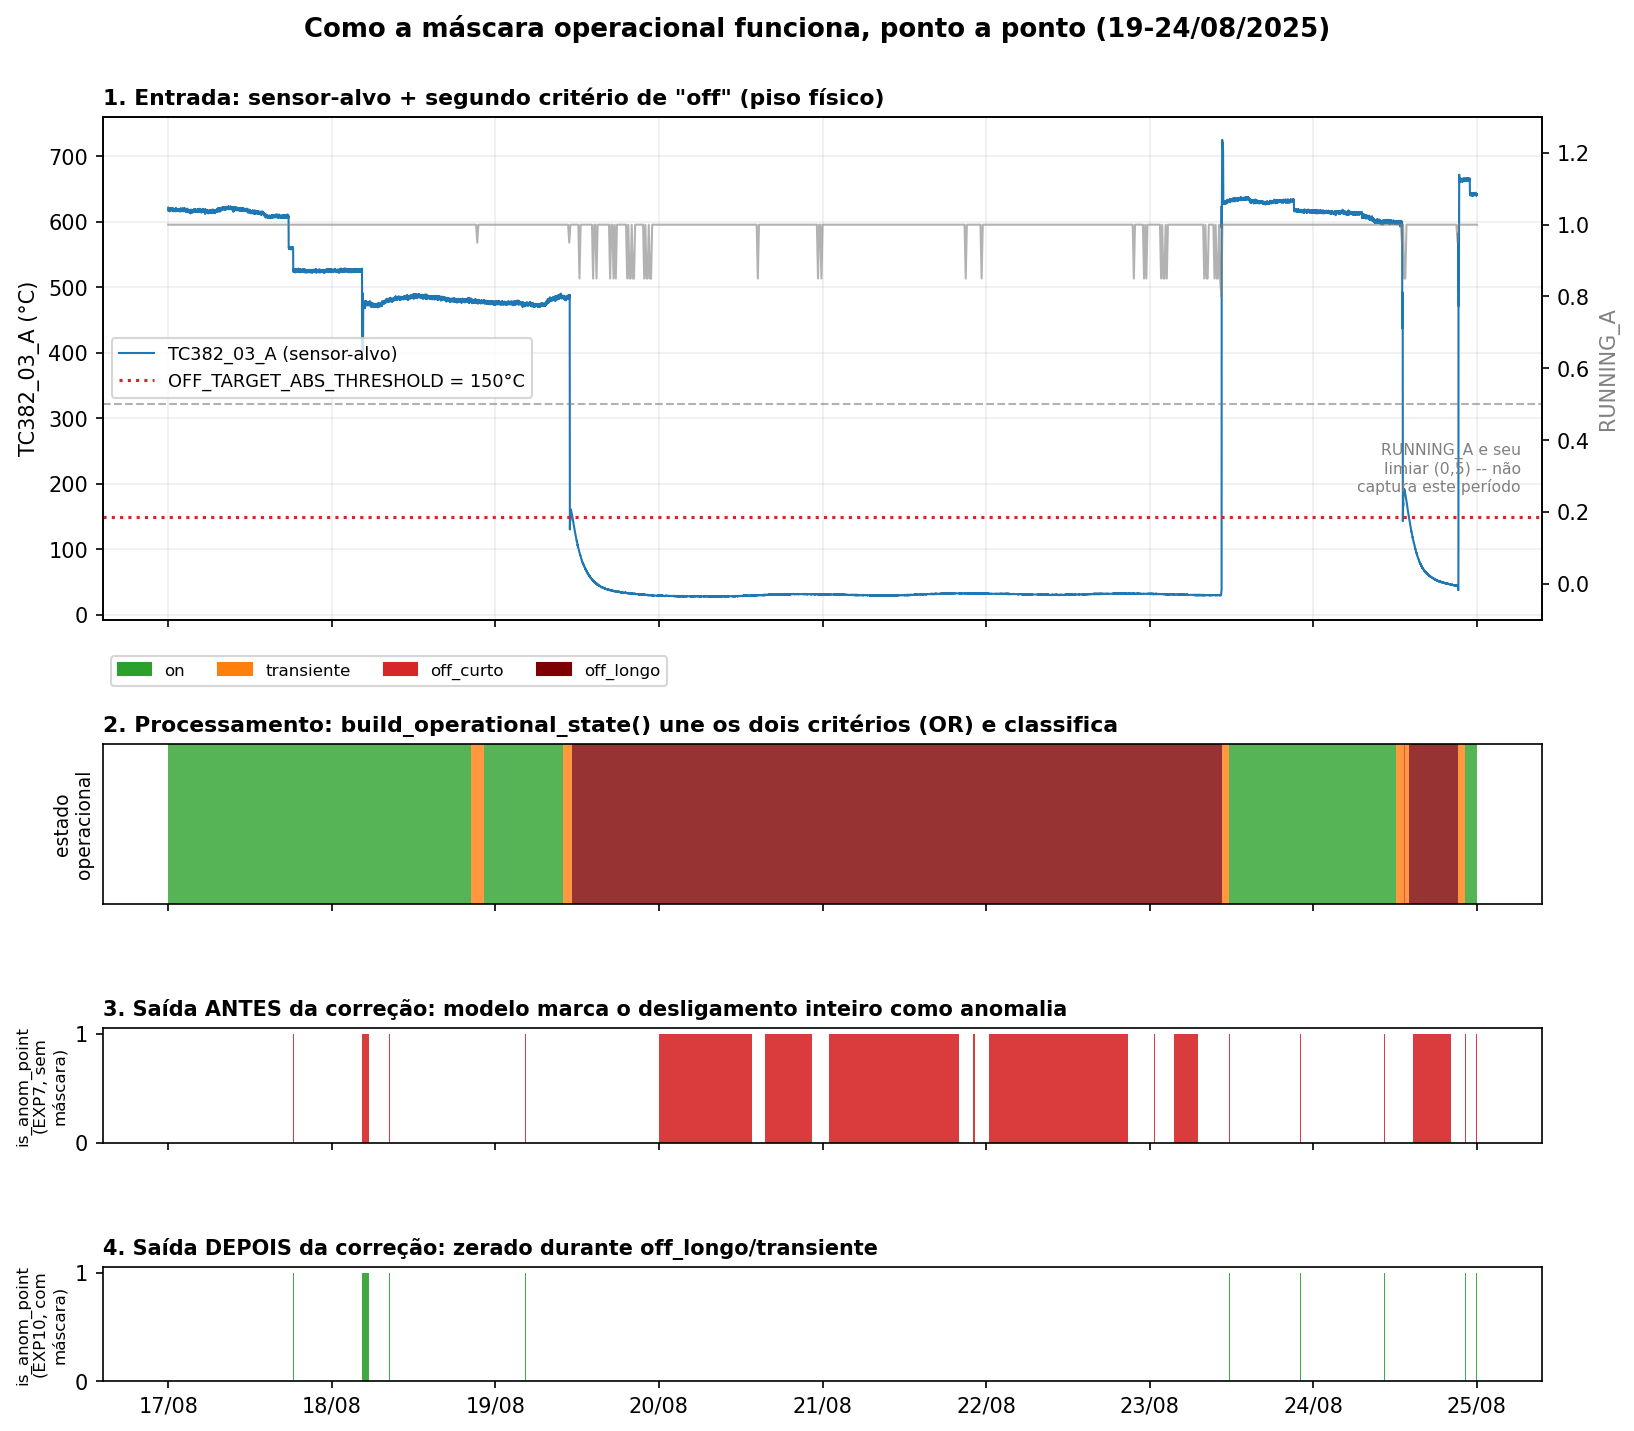
\includegraphics[width=\textwidth]{12_mecanismo_mascara_operacional.png}
\caption{A máscara operacional em ação, no episódio real do
Achado~1. \textbf{1:} o sensor-alvo cruza o piso de 150$^{\circ}$C
enquanto \texttt{RUNNING\_A} (cinza) permanece perto de 1 -- o critério
antigo sozinho nunca dispararia aqui. \textbf{2:} os dois critérios
unidos por OR classificam quase 3,5 dias como \texttt{off\_longo}
(vinho). \textbf{3:} sem a máscara, o modelo marca o desligamento
inteiro como anomalia (EXP7). \textbf{4:} com a máscara, esses pontos
são zerados (EXP10) -- só sobra o que acontece fora do período
\texttt{off}.}
\label{fig:mecanismo-mascara}
\end{figure}

\subsubsection*{Portão de rampa: taxa de variação suavizada de um proxy}

\texttt{apply\_load\_gate} (via \texttt{compute\_load\_ramp\_gate}) toma
uma série-proxy (\texttt{LOAD\_GATE\_SENSOR}, aqui \texttt{T5\_AVG\_A}),
suaviza com EWMA de meia-vida \texttt{LOAD\_GATE\_RAMP\_HALFLIFE\_MINUTES}
(causal --- só olha o passado), deriva no tempo para obter uma rampa em
unidades/hora, e toma o máximo trailing dessa rampa numa janela de
\texttt{LOAD\_GATE\_WINDOW\_MINUTES}. Bloqueia \texttt{is\_anom\_point}
quando esse máximo ultrapassa \texttt{LOAD\_GATE\_RAMP\_MAX}.

\begin{figure}[H]
\centering
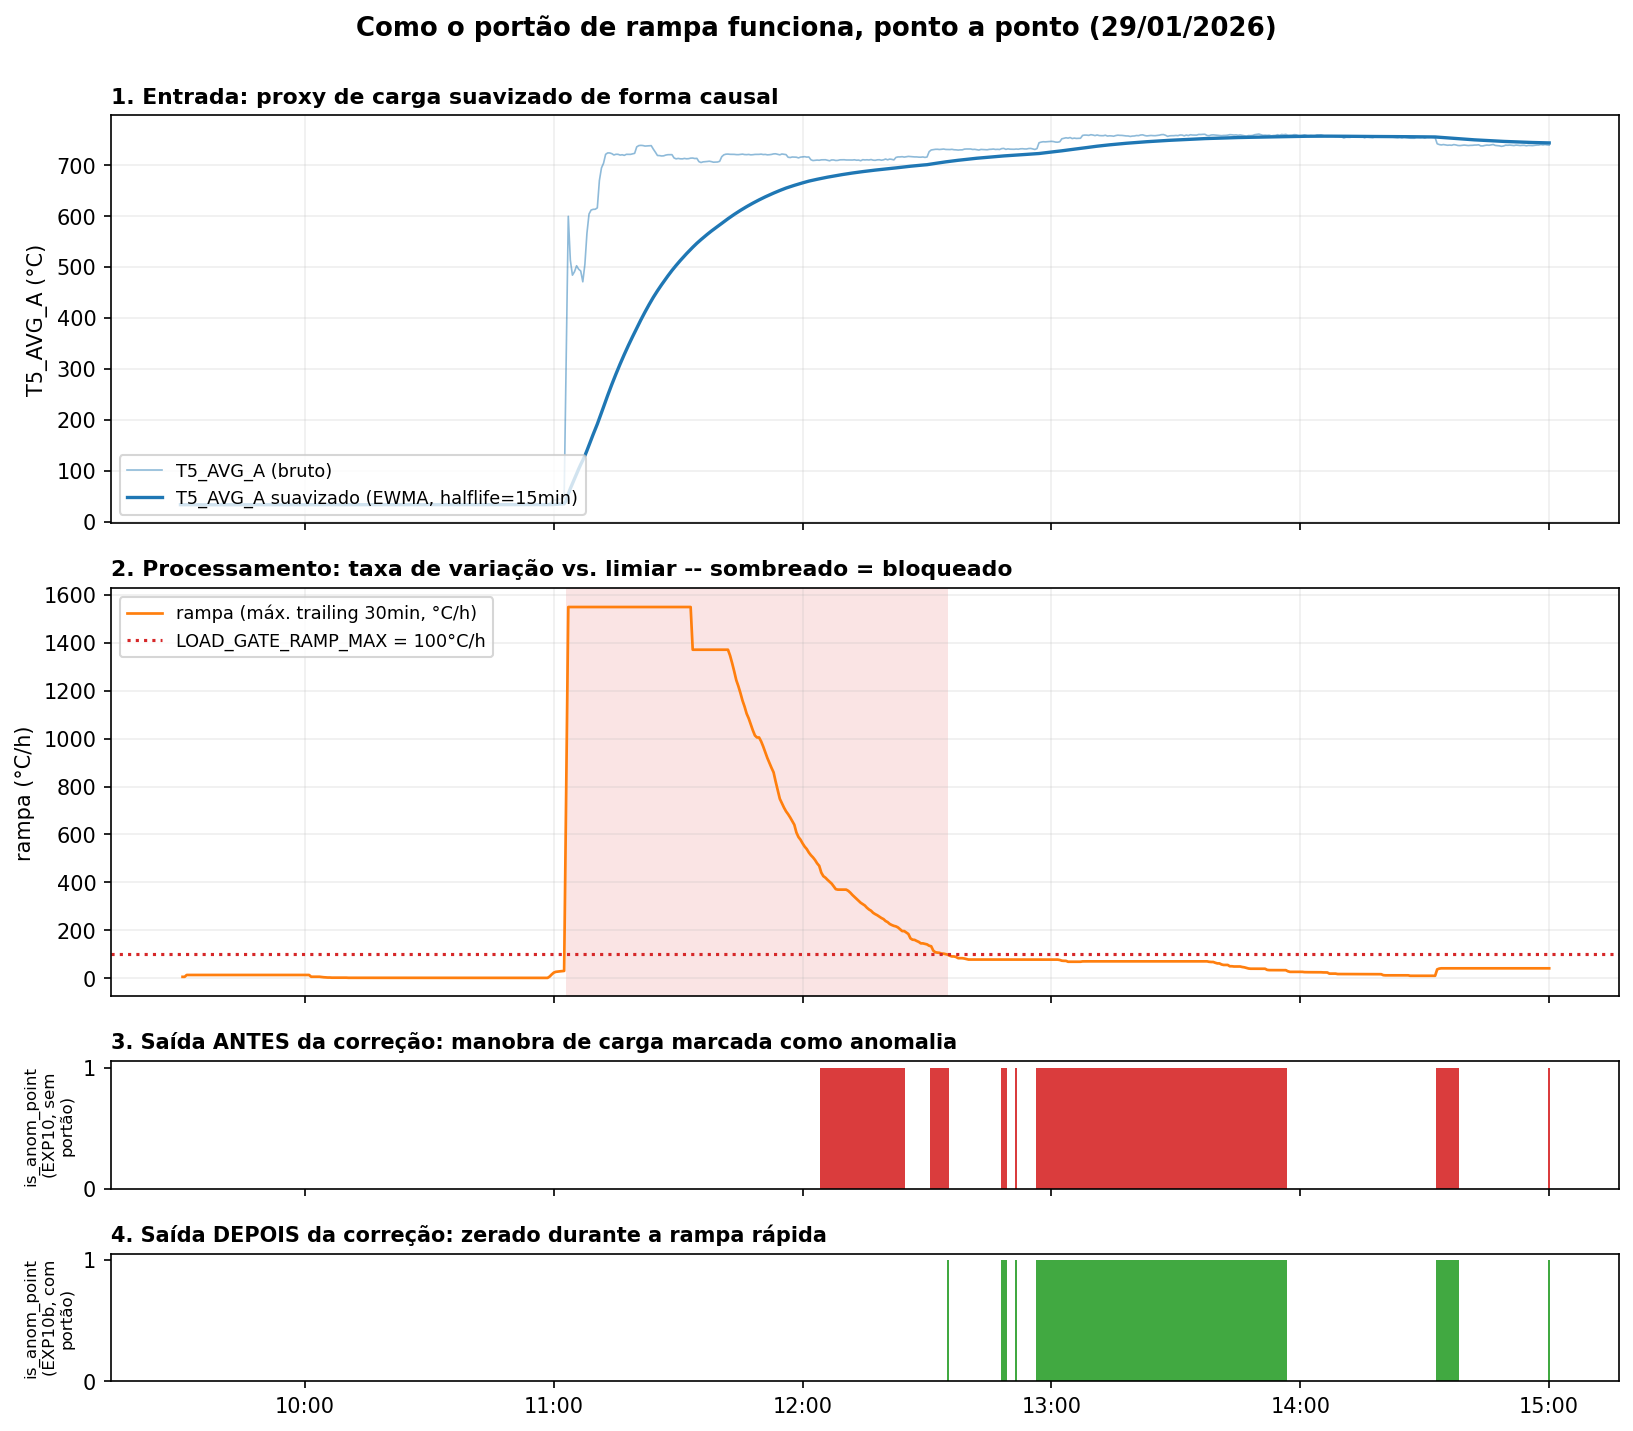
\includegraphics[width=\textwidth]{13_mecanismo_portao_rampa.png}
\caption{O portão de rampa em ação, num episódio real de manobra de
carga (29/01/2026). \textbf{1:} \texttt{T5\_AVG\_A} sobe $\sim$600$^{\circ}$C
em minutos; a curva suavizada (EWMA) segue com atraso controlado.
\textbf{2:} a rampa calculada dispara a mais de 1500$^{\circ}$C/h,
muito acima do limiar de 100 -- a área sombreada mostra exatamente
onde o portão fica ativo. \textbf{3:} sem o portão, o modelo marca a
manobra (e outros dois episódios não relacionados, fora da área
sombreada) como anomalia (EXP10). \textbf{4:} com o portão, só o
episódio \emph{dentro} da rampa some -- os outros dois, sem rampa
acentuada, continuam marcados (EXP10b), mostrando que o filtro é
seletivo, não um corte cego de horário.}
\label{fig:mecanismo-rampa}
\end{figure}

\subsubsection*{Portão de volatilidade: nível de um índice multivariado}

\texttt{apply\_volatility\_gate} (via \texttt{compute\_volatility\_index},
Seção~\ref{sec:achado3}) toma um conjunto de sensores
(\texttt{VOLATILITY\_GATE\_SENSORS}, aqui os 10 canais de vibração),
calcula o desvio-padrão móvel causal de cada um numa janela de
\texttt{VOLATILITY\_GATE\_WINDOW\_MINUTES} e reduz pela média entre
canais a cada instante. Bloqueia \texttt{is\_anom\_point} quando esse
índice ultrapassa \texttt{VOLATILITY\_GATE\_THRESHOLD} --- diferente do
portão de rampa, aqui o critério é o \emph{nível} do índice, não sua taxa
de variação (ver Seção~\ref{sec:achado3} para o porquê dessa escolha).

\begin{figure}[H]
\centering
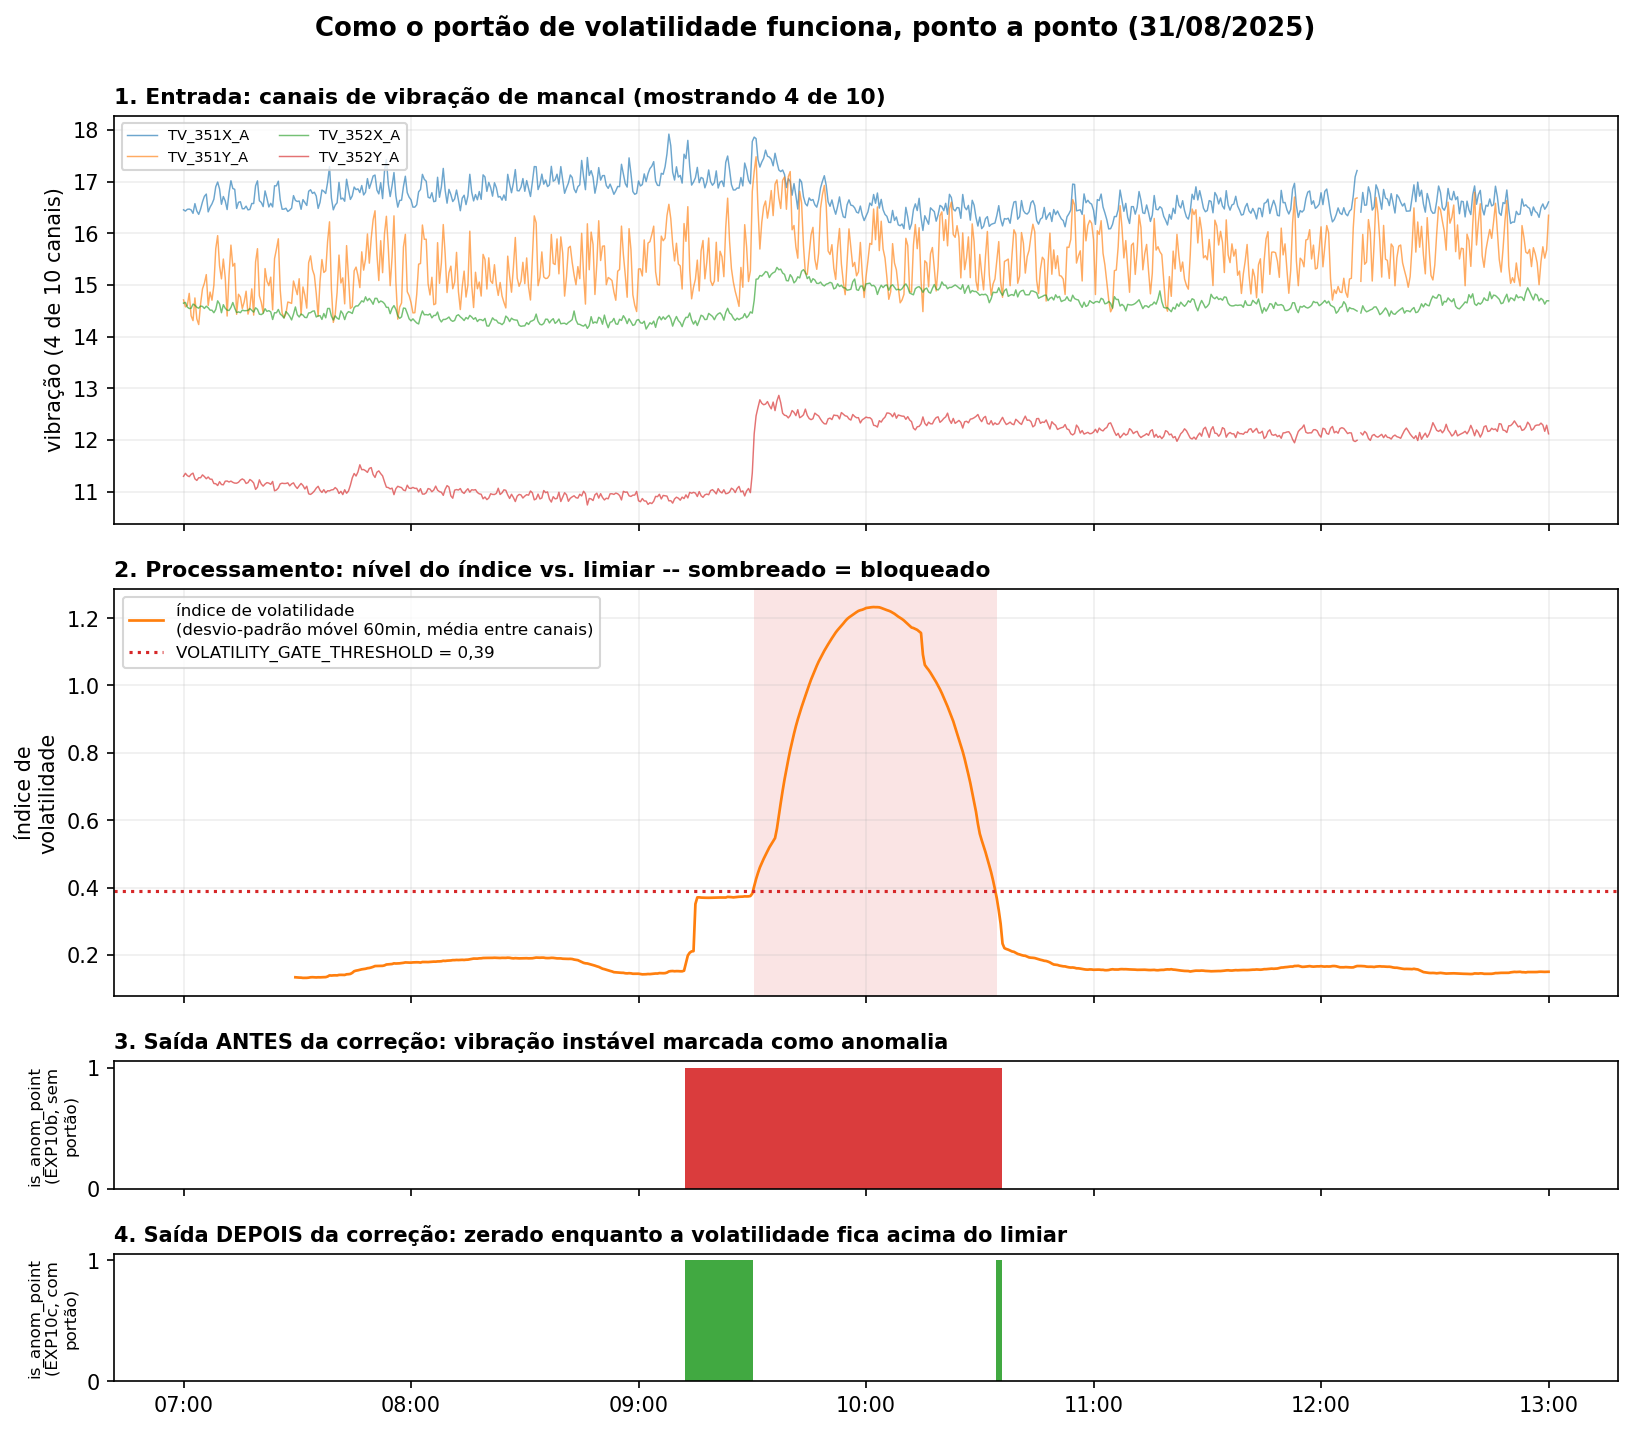
\includegraphics[width=\textwidth]{14_mecanismo_portao_volatilidade.png}
\caption{O portão de volatilidade em ação, no mesmo episódio de
31/08/2025 já visto na Figura~\ref{fig:rampa-exemplo}. \textbf{1:}
quatro dos 10 canais de vibração (o painel completo usa os 10) --
\texttt{TV\_352Y\_A} salta de patamar por volta das 09:10.
\textbf{2:} o índice de volatilidade (média do desvio-padrão móvel dos
10 canais) cruza o limiar de 0,39 logo depois e fica acima por
$\sim$1h20. \textbf{3:} sem o portão, o episódio inteiro é marcado como
anomalia (EXP10b). \textbf{4:} com o portão, a maior parte some -- só
sobram frações residuais bem nas bordas, exatamente onde o índice
cruza o limiar (o modelo já havia reagido um pouco antes/depois do
instante exato em que o índice passa a linha), evidência de que o
mecanismo está reagindo ponto a ponto, não arredondando por episódio
inteiro.}
\label{fig:mecanismo-volatilidade}
\end{figure}

\subsection{Diagnóstico: fragmentar em vez de agregar}

A ideia central deste trabalho, difere do que fizemos até aqui: em vez de
olhar só o \texttt{normal\_alert\_rate} agregado, \textbf{fragmentamos a
série de \texttt{is\_anom\_point} em episódios contínuos} (agrupando
pontos anômalos consecutivos com gap $\leq$5 min) e cruzamos cada
episódio com:

\begin{enumerate}[label=(\alph*)]
  \item os dados brutos de \texttt{TC382\_03\_A}/\texttt{T5\_AVG\_A} e
        dos 10 canais de vibração, no período do episódio e ao redor;
  \item o catálogo completo de alarmes (47 tags, não só os 2 sensores
        avaliados) --- pra checar se o episódio coincide com \emph{algum}
        evento real registrado em outro lugar da planta;
  \item o estado operacional (\texttt{RUNNING\_A}) computado pela
        máscara existente.
\end{enumerate}

Essa abordagem revelou uma estrutura que a métrica agregada escondia:
dos 12.782 pontos de falso alerta no período OOS, \textbf{72,5\% se
concentram em apenas 10 episódios} de 295 no total. Não é ruído
espalhado --- é um número pequeno de causas concretas e investigáveis.

\begin{figure}[H]
\centering
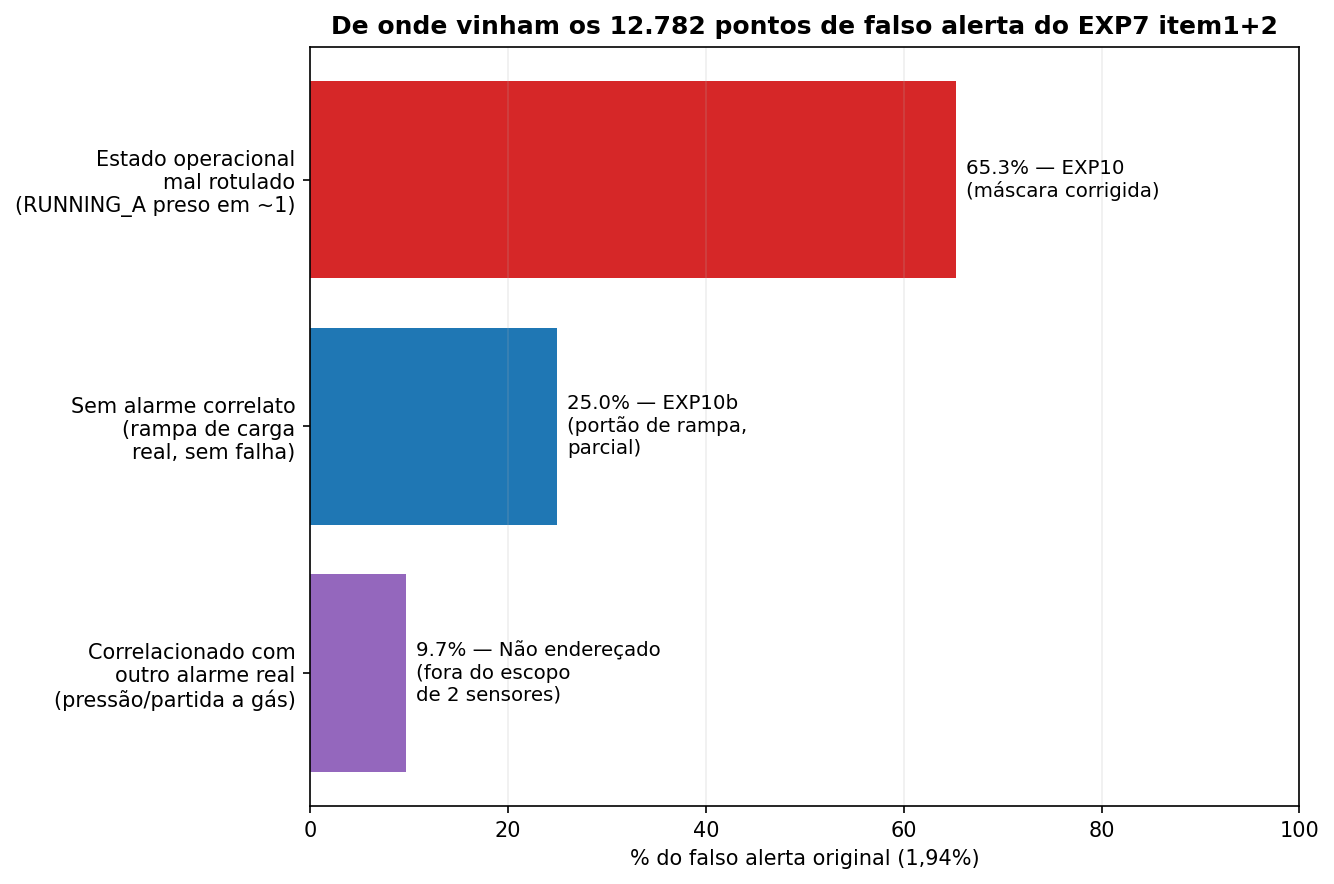
\includegraphics[width=0.9\textwidth]{02_decomposicao_causas_fp.png}
\caption{Decomposição dos 12.782 pontos de falso alerta por causa raiz,
depois de investigar os episódios individualmente.}
\end{figure}

% =====================================================================
\section{Achado 1: desligamento real que a máscara não via}
\label{sec:achado1}
% =====================================================================

\subsection{O episódio}

Os 5 maiores episódios (61,5\% de todo o falso alerta) caem todos entre
19 e 24 de agosto de 2025. Ao puxar a série bruta:
\texttt{TC382\_03\_A} despenca de $\sim$478$^{\circ}$C para
\textbf{$\sim$28--32$^{\circ}$C} (nível ambiente) e fica lá por
\textbf{3,5 dias}. Fisicamente incompatível com operação --- faixa normal
é $\sim$600--800$^{\circ}$C.

O problema: \texttt{RUNNING\_A} (o sensor de referência da máscara
operacional) fica em $\sim$0,96--1,0 o tempo todo durante esse período.
A máscara original só olha \texttt{RUNNING\_A} $\leq$ 0,5 pra decidir
``desligado'' --- então esse desligamento inteiro nunca era excluído da
avaliação, e o modelo (corretamente!) marcando temperatura fora de
qualquer faixa treinada como anomalia virava, na nossa métrica, ``falso''
alerta.

\begin{figure}[H]
\centering
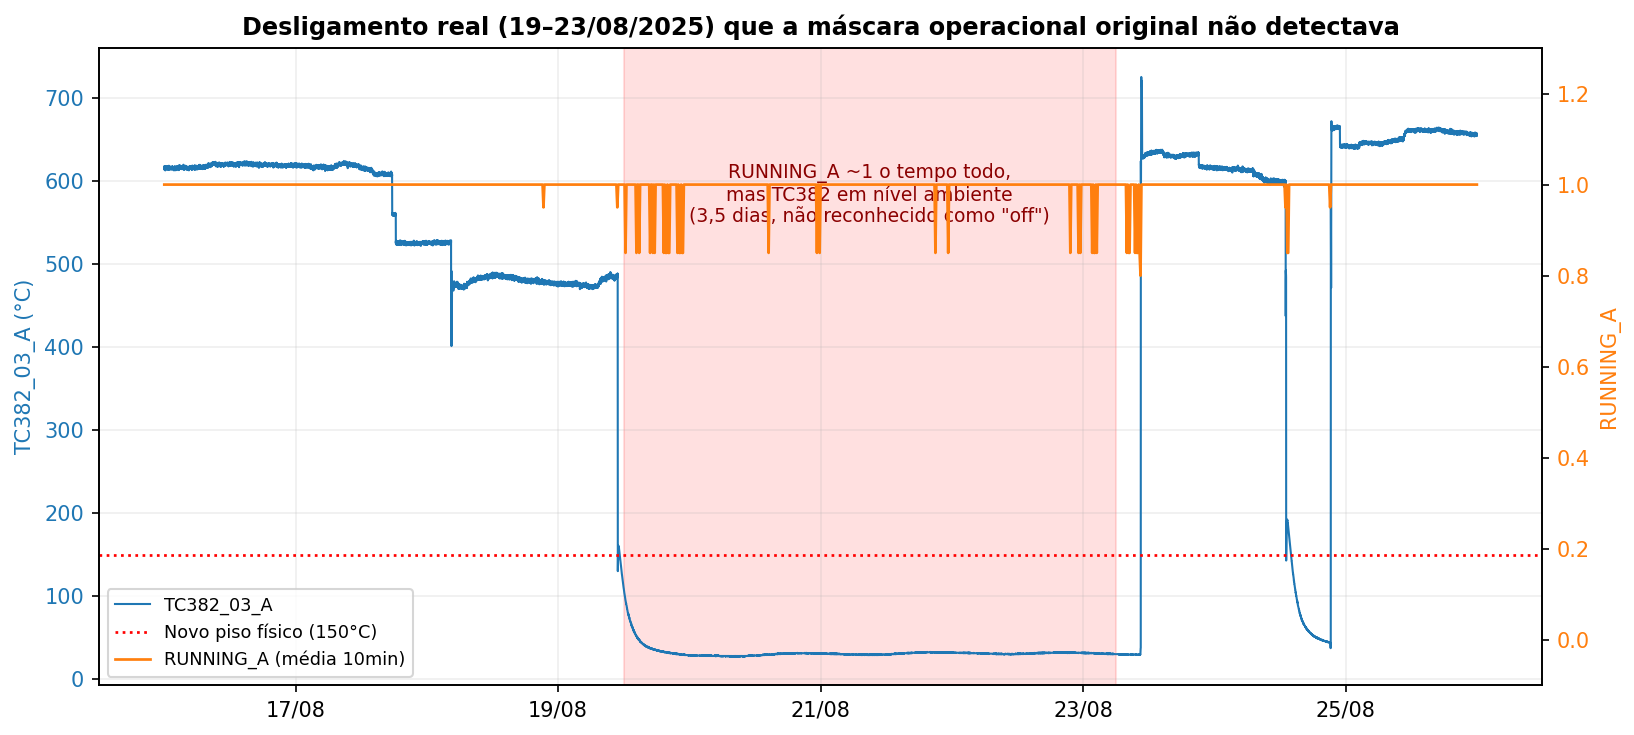
\includegraphics[width=\textwidth]{03_desligamento_mal_rotulado.png}
\caption{\texttt{TC382\_03\_A} cai a nível ambiente por 3,5 dias enquanto
\texttt{RUNNING\_A} permanece $\sim$1. A área sombreada é o período que a
máscara original classificava como ``on''.}
\end{figure}

\subsection{Confirmação: não é artefato de dado}

Cruzando com o catálogo completo de 47 tags: \texttt{PI\_6240319\_AL}
(falha de partida a gás) dispara em 19/08 e novamente em 23/08;
\texttt{PAL\_6240315} (pressão baixa de gás combustível) dispara em
23/08 --- exatamente nas bordas do período. Desligamento e religamento
reais, documentados, não uma falha de sensor.

\subsection{Correção: segundo critério de ``off'' independente}

\texttt{build\_operational\_state} (\texttt{scoring.py}) ganhou um
parâmetro opcional \texttt{secondary\_series}/
\texttt{secondary\_off\_abs\_threshold}: o próprio sensor-alvo do grupo
(\texttt{TC382\_03\_A}) caindo abaixo de um piso físico (150$^{\circ}$C
--- bem abaixo de qualquer operação normal, com folga sobre os
$\sim$28--32$^{\circ}$C do desligamento confirmado) \textbf{também} conta
como ``off'', unido (OR) ao critério de \texttt{RUNNING\_A} antes da
classificação off\_curto/off\_longo/transiente --- reusando toda a lógica
de detecção de corrida contínua já existente, sem duplicar código. Novo
campo de config: \texttt{OFF\_TARGET\_ABS\_THRESHOLD}.

\textbf{Por que isso é a correção certa e não um ajuste ad-hoc:} o
critério original (\texttt{RUNNING\_A}) e o novo (piso físico do alvo)
são \emph{independentes} --- um poderia falhar sem o outro falhar junto.
Unir os dois com OR é estritamente mais seguro que qualquer um sozinho,
sem introduzir nenhuma suposição nova sobre o que é ``normal''.

\subsection{Resultado (EXP10)}

\begin{table}[H]
\centering
\begin{tabular}{@{}lcc@{}}
\toprule
\textbf{Métrica} & \textbf{EXP7 item1+2} & \textbf{EXP10 (+ máscara corrigida)} \\
\midrule
hit\_rate (40 alarmes) & 92,5\% (37/40) & \textbf{92,5\% (37/40)} \\
Falso alerta & 1,94\% & \textbf{0,67\%} \\
\bottomrule
\end{tabular}
\caption{Zero mudança de detecção, falso alerta cai quase 3x. Seed-sweep
(5 sementes) confirma estabilidade: desvio-padrão de 0,019pp.}
\end{table}

% =====================================================================
\section{Um caminho testado e descartado: debounce}
\label{sec:debounce}
% =====================================================================

Antes de investigar o restante do falso alerta em detalhe, testamos a
alavanca mais óbvia: aumentar o \texttt{debounce} (exigir mais pontos
anômalos consecutivos antes de disparar o alerta). Como o candidato usa
debounce=1, o \texttt{is\_anom\_point} já cacheado é o sinal bruto ---
deu pra simular toda a grade offline, sem re-rodar remoto.

\begin{figure}[H]
\centering
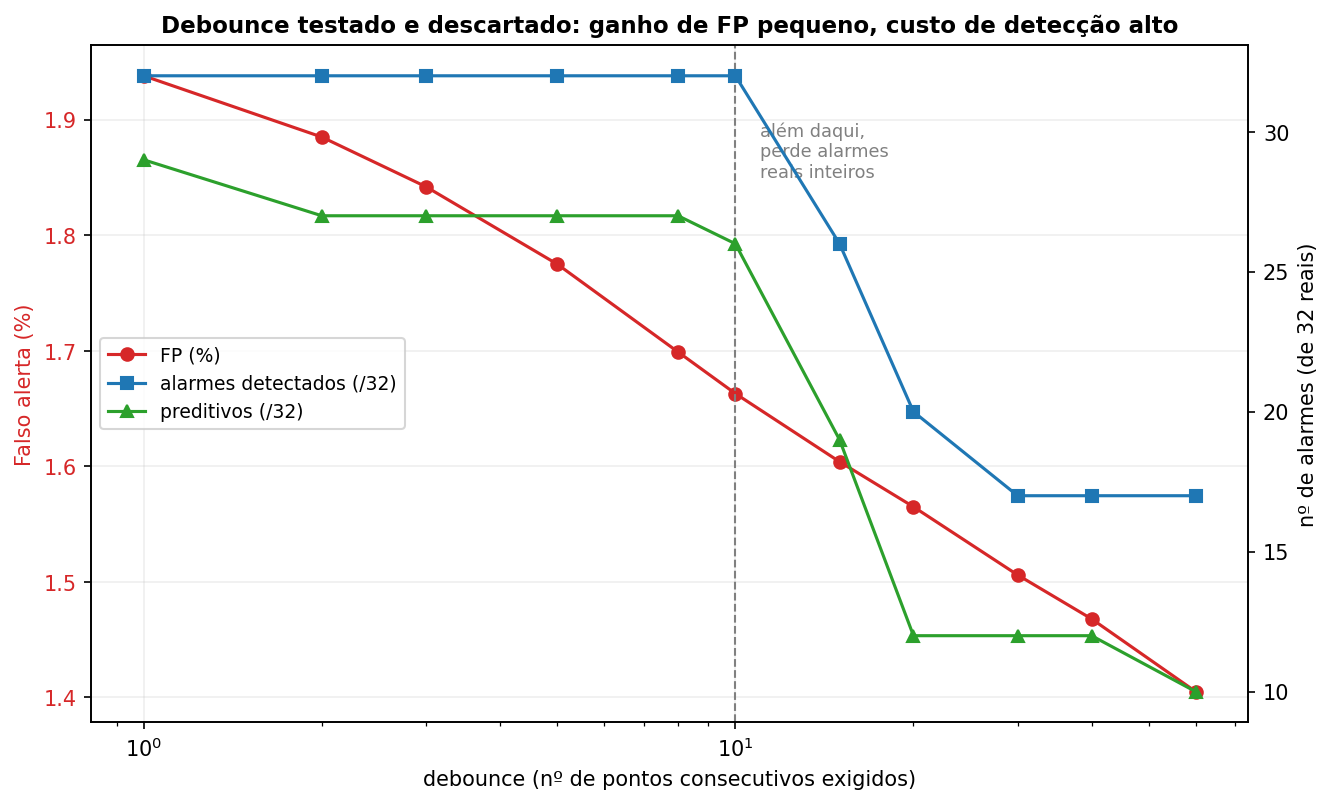
\includegraphics[width=0.85\textwidth]{06_grade_debounce_descartada.png}
\caption{Até debounce=10 o ganho de FP é pequeno (1,94\%$\to$1,66\%) e já
custa 3 casos preditivos. Além disso, o modelo começa a perder alarmes
reais inteiros.}
\end{figure}

\textbf{Por que não funciona:} os episódios de falso alerta residual têm
mediana de 6 pontos/2,5 minutos de duração --- quase idêntico à duração
dos episódios mais curtos que ainda assim precedem um alarme real (25º
percentil = 6 min). Debounce não consegue separar os dois porque as
distribuições de duração se sobrepõem.

\begin{figure}[H]
\centering
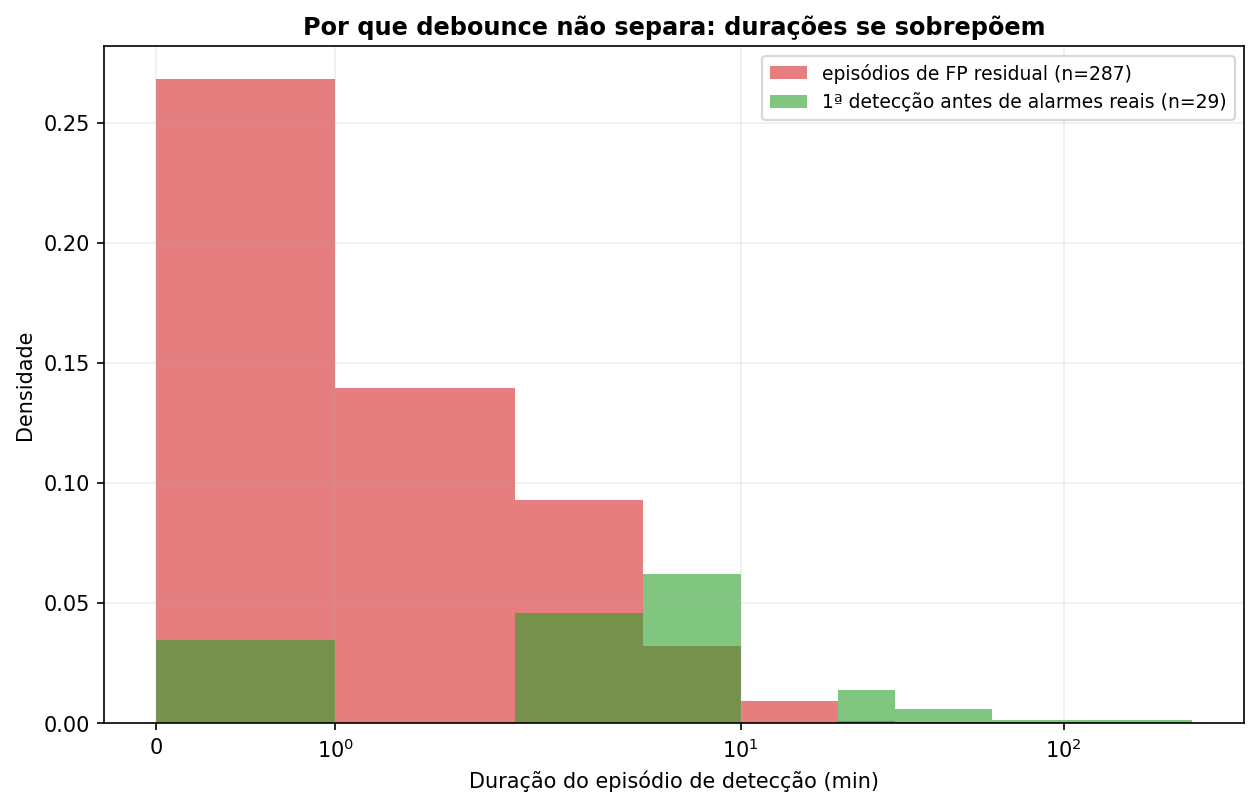
\includegraphics[width=0.85\textwidth]{05_duracao_episodios_fp_vs_real.png}
\caption{Duração dos episódios de falso alerta residual (vermelho) vs.
duração do episódio que gera a 1ª detecção antes de cada alarme real
(verde). Sobreposição forte nas durações curtas.}
\end{figure}

Esse é um achado negativo documentado por completude, consistente com a
lição já registrada no EXP7: mexer em limiar/debounce agressivamente
sempre trocou detecção real por FP de forma desfavorável.

% =====================================================================
\section{Achado 2: rampas de carga reais}
\label{sec:achado2}
% =====================================================================

\subsection{Investigação dos 10 maiores episódios residuais}

Com o desligamento de agosto resolvido, sobravam 4.441 pontos de falso
alerta em 287 episódios. Uma primeira caracterização estatística já
apontava a direção: \textbf{o nível de \texttt{TC382\_03\_A} é igual}
entre pontos de falso alerta e pontos normais (não é viés de faixa), mas
a \textbf{variabilidade local é 5--9x maior} (desvio-padrão de 1h:
5,37 vs. 1,09 nos pontos normais; vibração $\sim$2,5x mais volátil).

Investigando os 10 maiores episódios individualmente (dados brutos, não
só estatística agregada): \textbf{8 de 10} mostram o mesmo padrão ---
\texttt{TC382\_03\_A}/\texttt{T5\_AVG\_A} subindo ou caindo dezenas de
graus em cerca de 1 hora, com o desvio-padrão da vibração triplicando ou
sextuplicando durante o episódio. Sem alarme, sem falha --- manobra de
carga real.

\begin{figure}[H]
\centering
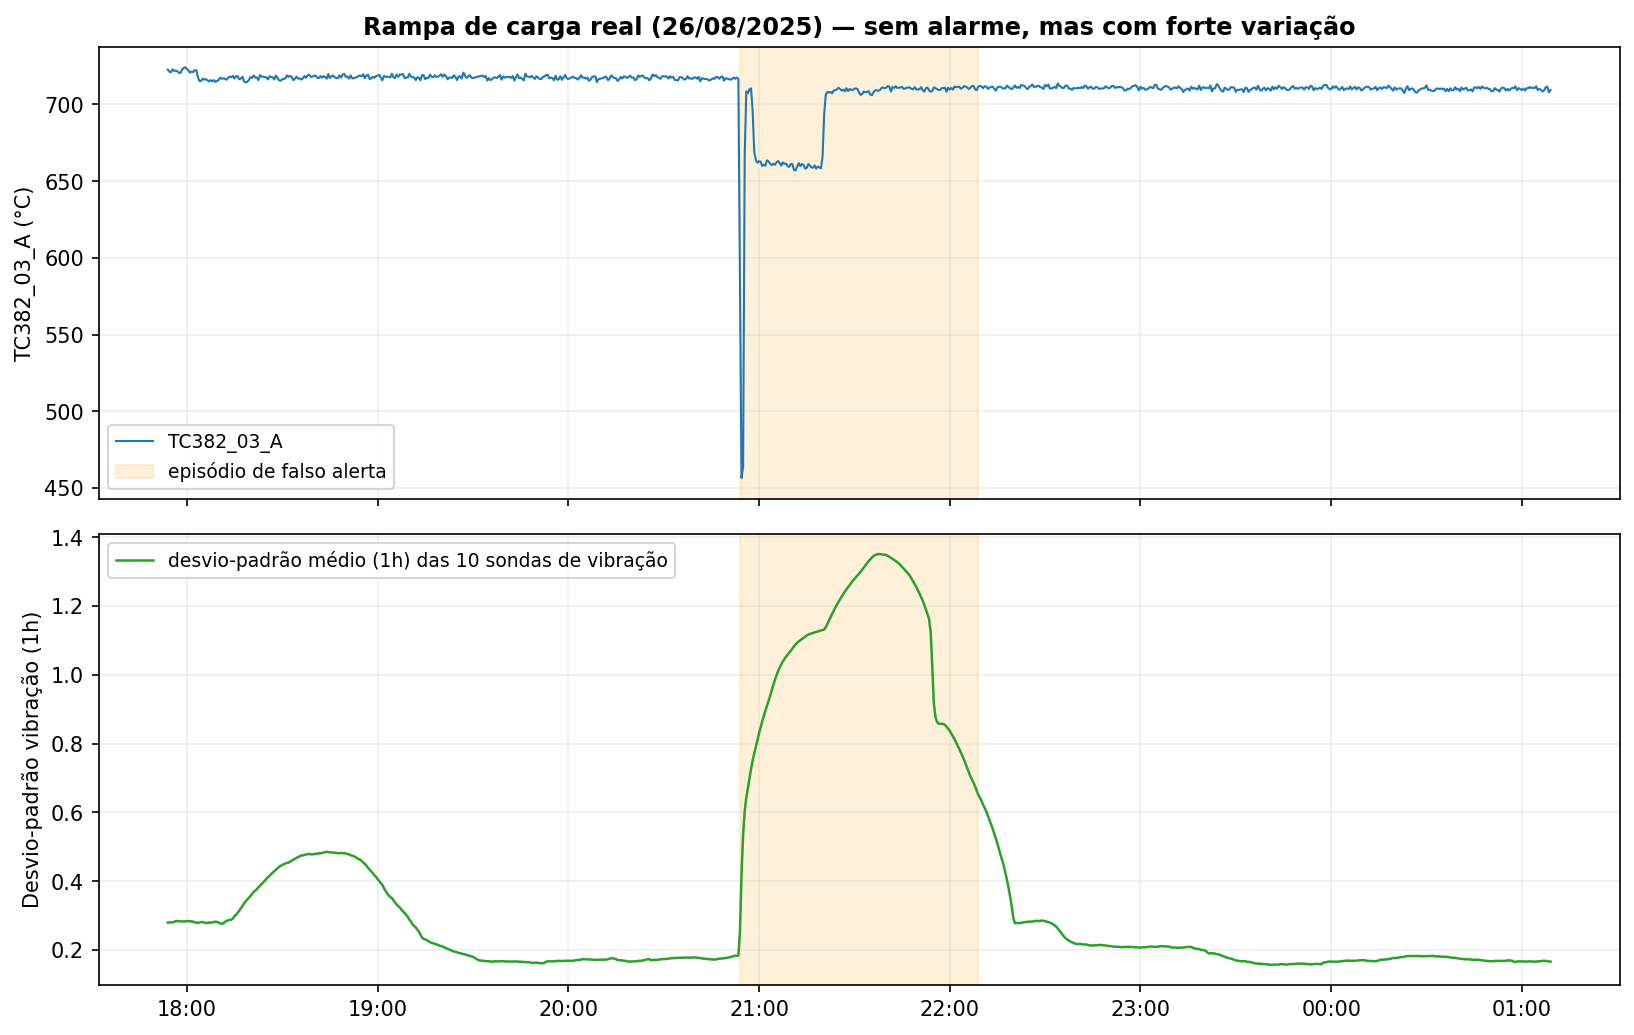
\includegraphics[width=\textwidth]{04_rampa_carga_exemplo.png}
\caption{Exemplo (26/08/2025): queda e recuperação de $\sim$60$^{\circ}$C
em $\sim$1h30, com desvio-padrão de vibração subindo de $\sim$0,17 para
$\sim$1,35 (8x) \emph{e permanecendo elevado} por boa parte do episódio ---
o padrão que motiva o portão de volatilidade da Seção~\ref{sec:achado3}.}
\label{fig:rampa-exemplo}
\end{figure}

\subsection{A correção já existia --- só não estava conectada}

O pipeline CNN1D-AE (\texttt{pipeline.py}) já tinha um ``portão de rampa
de carga'' (\texttt{ENABLE\_LOAD\_GATE}/\texttt{apply\_load\_gate}):
suprime \texttt{is\_anom\_point} quando a rampa (derivada suavizada) de
um sensor-proxy de carga ultrapassa um limite, de forma causal (nunca
olha o futuro). Mecanismo certo para exatamente esse padrão --- mas
\textbf{nunca tinha sido portado para o pipeline AutoML}, que é o que
usamos desde o EXP5.

\subsection{Ajuste: por que a janela curta importa}

A primeira tentativa, com os parâmetros default do CNN1D-AE
(\texttt{halflife}=120min, janela trailing=360min), \textbf{custou
detecção real} --- bloqueava até 6 dos 29 casos preditivos, porque uma
rampa de temperatura de falha genuína tem a mesma assinatura de taxa de
variação que uma rampa de carga legítima; uma janela de memória longa
não distingue as duas. Reduzindo a janela (\texttt{halflife}=15min,
trailing=30min) e testando o limiar \texttt{ramp\_max} por simulação
offline:

\begin{figure}[H]
\centering
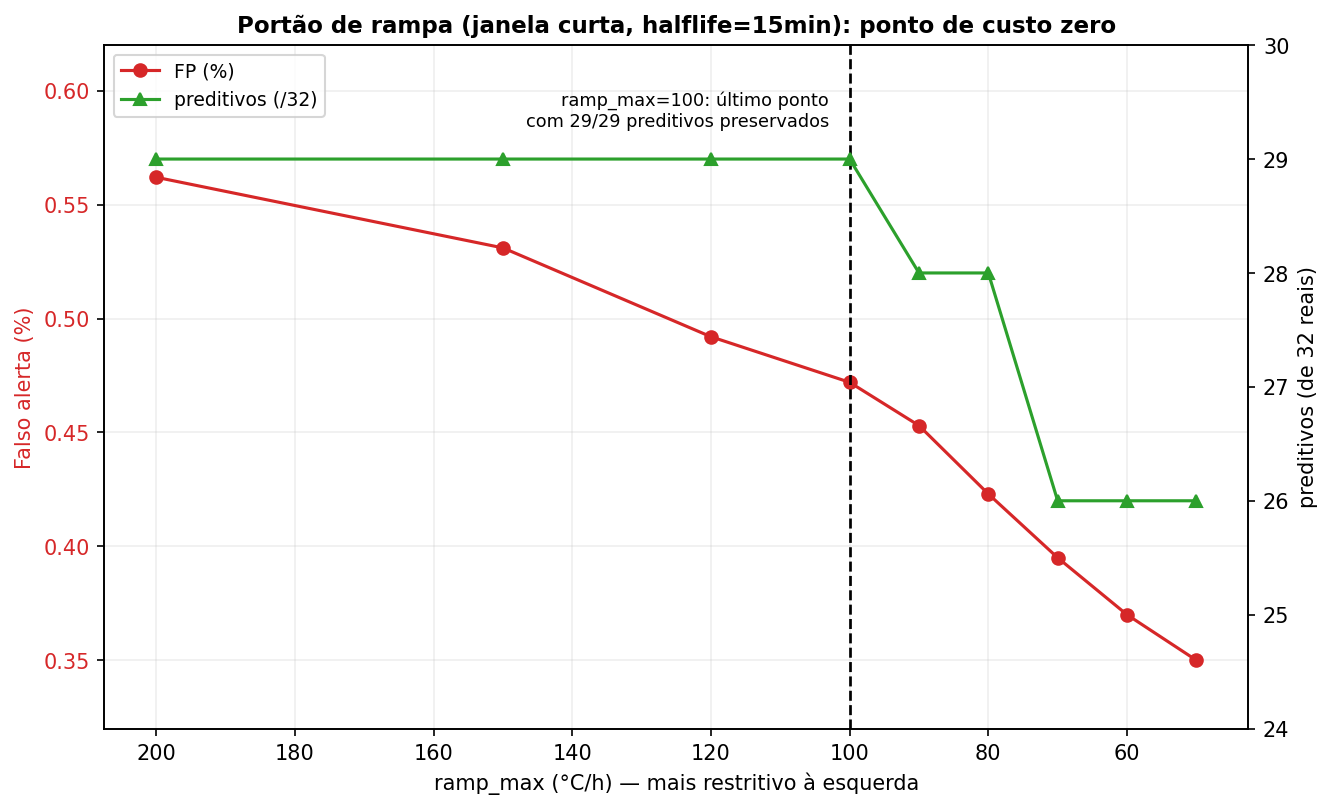
\includegraphics[width=0.85\textwidth]{07_portao_rampa_ramp_max.png}
\caption{Com janela curta, \texttt{ramp\_max=100}$^{\circ}$C/h é o ponto
exato de custo zero: último valor que preserva os 29/29 casos
preditivos.}
\end{figure}

\subsection{Resultado (EXP10b)}

\begin{table}[H]
\centering
\begin{tabular}{@{}lccc@{}}
\toprule
\textbf{Métrica} & \textbf{EXP7 item1+2} & \textbf{EXP10} & \textbf{EXP10b (+ portão de rampa)} \\
\midrule
hit\_rate (40 alarmes) & 92,5\% (37/40) & 92,5\% (37/40) & \textbf{92,5\% (37/40)} \\
Falso alerta & 1,94\% & 0,67\% & \textbf{0,48\%} \\
\bottomrule
\end{tabular}
\caption{Novamente zero mudança de detecção. Seed-sweep confirma
estabilidade (desvio-padrão de 0,016pp).}
\end{table}

% =====================================================================
\section{Achado 3: volatilidade que persiste, não que sobe}
\label{sec:achado3}
% =====================================================================

O portão de rampa (Seção~\ref{sec:achado2}) reagiu bem à parte das
rampas de carga que se manifestam como uma variação clara de
\emph{nível} em \texttt{T5\_AVG\_A}. Mas ele não foi desenhado pensando
na vibração --- e o padrão que já tínhamos visto na
Figura~\ref{fig:rampa-exemplo} (Seção~\ref{sec:achado2}) é diferente: o
desvio-padrão da vibração \emph{sobe} durante a manobra, mas também
\emph{permanece} elevado por 1--2h, não é só um pico passageiro na
subida.

\subsection{Tentativa 1: reaproveitar o portão de rampa (falhou)}

A primeira tentativa foi a mais óbvia: alimentar
\texttt{apply\_load\_gate} com um índice de volatilidade de vibração
(desvio-padrão móvel médio entre os 10 canais) no lugar do proxy de
temperatura, mantendo o mesmo mecanismo de taxa de variação. O resultado
foi decepcionante --- o ponto de custo zero (\texttt{thr=8}, preservando
29/29 preditivos) reduzia o FP de 0,480\% para apenas 0,477\%, e
qualquer limiar que desse um ganho real custava 2 casos preditivos em
praticamente toda a faixa testada (painel esquerdo da
Figura~\ref{fig:portao-volatilidade}).

\textbf{Por quê:} taxa de variação mede o quão rápido algo está mudando
\emph{agora}, e tanto o início de uma rampa de carga real quanto o
início de uma escalada genuína de falha aceleram a volatilidade de forma
parecida --- o mesmo problema de assinatura compartilhada que já tinha
custado detecção na primeira tentativa do portão de rampa
(Seção~\ref{sec:achado2}), agora reaparecendo por um motivo relacionado
mas distinto: a métrica escolhida (derivada) não é a que separa os dois
casos.

\subsection{Tentativa 2: limiar direto no nível (funcionou)}

Reformulando pra medir o que a Figura~\ref{fig:rampa-exemplo} realmente
mostrava --- não a taxa de subida, mas o \emph{nível} sustentado ---
implementamos \texttt{compute\_volatility\_index}/
\texttt{apply\_volatility\_gate} (\texttt{scoring.py}): desvio-padrão
móvel causal (\texttt{VOLATILITY\_GATE\_WINDOW\_MINUTES}=60min) de cada
um dos 10 canais de vibração, reduzido pela média entre canais a cada
instante, bloqueando \texttt{is\_anom\_point} sempre que esse índice
ultrapassa um limiar fixo (não uma taxa). Testado por simulação offline
sobre o já corrigido pelo EXP10b:

\begin{figure}[H]
\centering
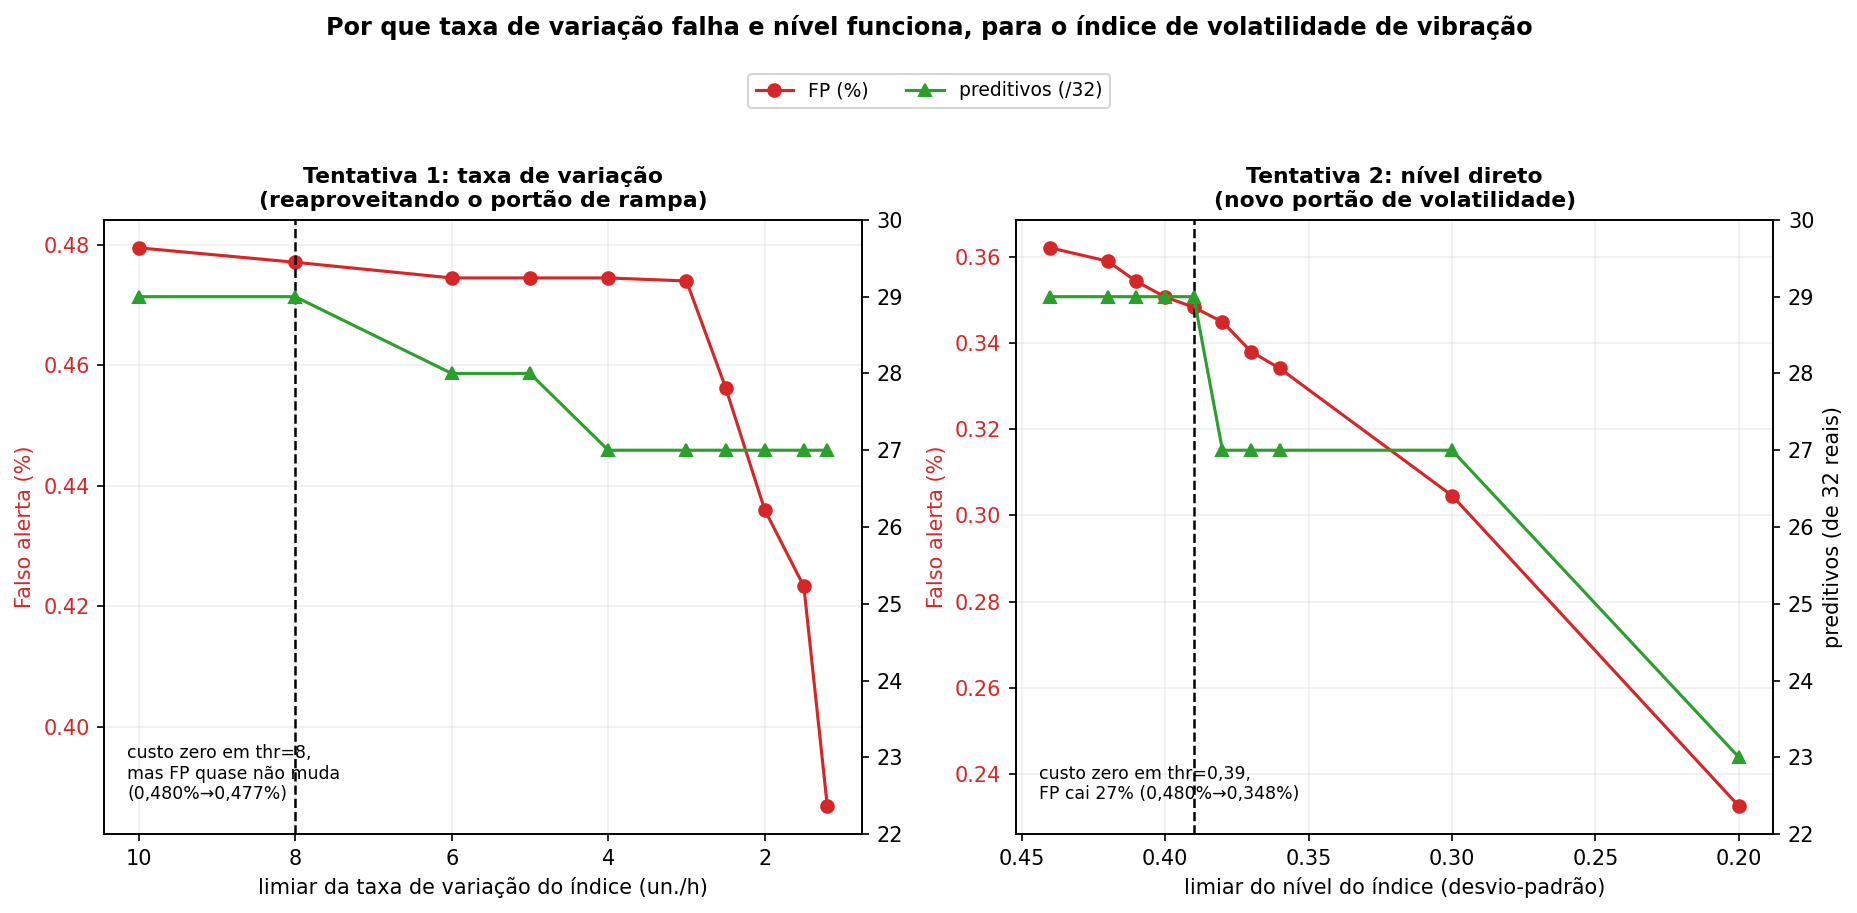
\includegraphics[width=\textwidth]{10_portao_volatilidade_comparacao.png}
\caption{Painel esquerdo: taxa de variação do índice de volatilidade ---
o ponto de custo zero mal reduz o FP. Painel direito: limiar direto no
nível do mesmo índice --- \texttt{threshold=0,39} preserva 29/29
preditivos com queda real de FP (27\% relativo).}
\label{fig:portao-volatilidade}
\end{figure}

\subsection{Resultado (EXP10c)}

\begin{table}[H]
\centering
\begin{tabular}{@{}lcccc@{}}
\toprule
\textbf{Métrica} & \textbf{EXP7 item1+2} & \textbf{EXP10} & \textbf{EXP10b} & \textbf{EXP10c (+ portão de volatilidade)} \\
\midrule
hit\_rate (40 alarmes) & 92,5\% (37/40) & 92,5\% (37/40) & 92,5\% (37/40) & \textbf{92,5\% (37/40)} \\
Falso alerta & 1,94\% & 0,67\% & 0,48\% & \textbf{0,35\%} \\
\bottomrule
\end{tabular}
\caption{Quarta confirmação seguida de custo zero de detecção.
Seed-sweep: desvio-padrão de 0,011pp.}
\end{table}

% =====================================================================
\section{Resultado consolidado}
% =====================================================================

\begin{figure}[H]
\centering
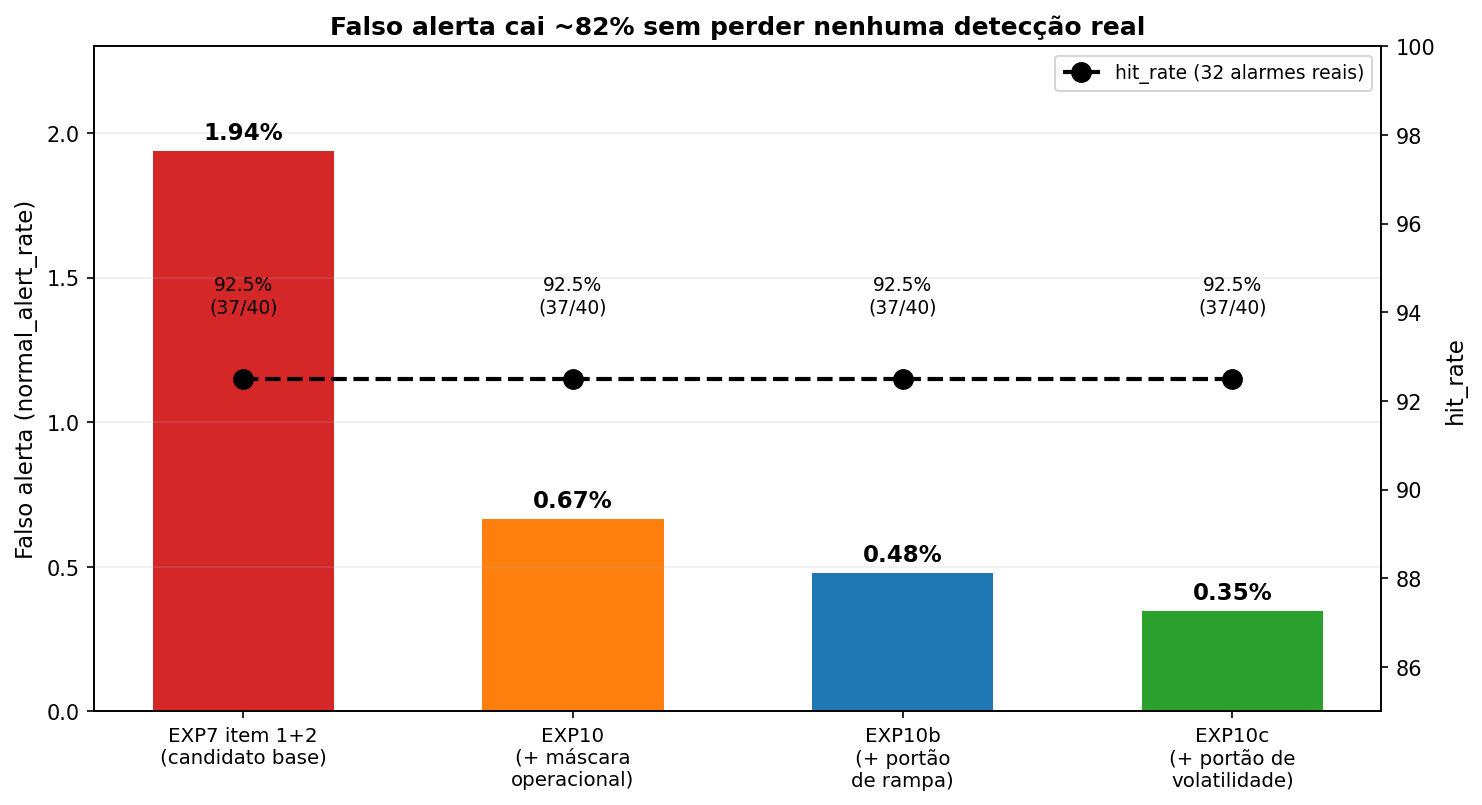
\includegraphics[width=0.95\textwidth]{01_fp_vs_hitrate_evolucao.png}
\caption{Falso alerta cai $\sim$82\% (1,94\%$\to$0,35\%) ao longo das
três correções, com hit\_rate idêntico (92,5\%, 37/40) em todas as
etapas.}
\end{figure}

\subsection{A jornada completa: da detecção ao falso alerta}

O relatório do EXP7 multiescala (\texttt{relatorio\_exp7\_multiescala.pdf})
mostrava a evolução de \texttt{Preditivo}/\texttt{Reativo}/\texttt{Sem
detecção} ao longo de EXP6 $\to$ item 1 $\to$ item 1+2 -- a fase em que
\emph{a detecção} melhorou. Este relatório continua exatamente dali, mas
numa fase diferente: da EXP7 item 1+2 em diante, a detecção já não muda
mais (os mesmos 29 preditivos, 8 reativos, 3 sem detecção se repetem
idênticos em EXP10, EXP10b e EXP10c) -- o que evolui é só o falso alerta.
A Figura~\ref{fig:evolucao-completa} junta as duas fases num único
gráfico, deixando visível a virada: as barras (detecção) sobem entre as
duas primeiras colunas e depois ficam paradas; a linha (falso alerta)
seguiu praticamente estável entre as duas primeiras e despenca na
terceira.

\begin{figure}[H]
\centering
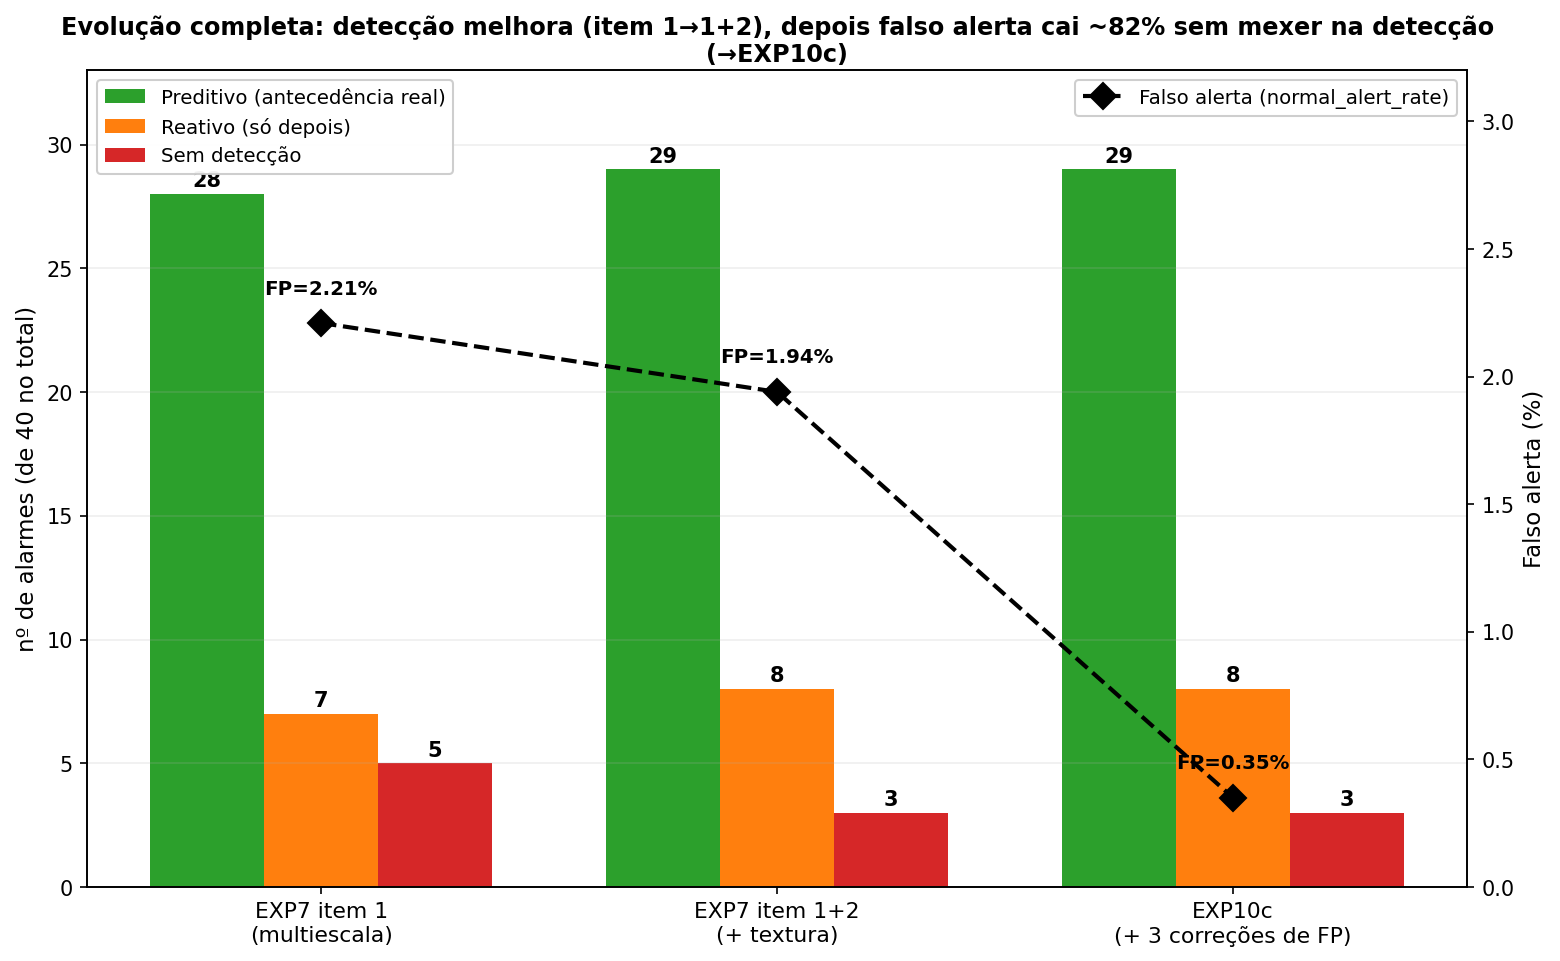
\includegraphics[width=\textwidth]{15_evolucao_completa_deteccao_fp.png}
\caption{Evolução completa: EXP7 item 1 $\to$ item 1+2 (ganho de
detecção, achado do relatório anterior) $\to$ EXP10c (ganho de falso
alerta, achado deste relatório). Barras = alarmes por categoria (eixo
esquerdo); linha tracejada = falso alerta (eixo direito). As barras
verde/laranja/vermelha ficam \emph{idênticas} entre item 1+2 e EXP10c --
prova visual de que as três correções de FP não mexeram em nenhuma
detecção, só na linha preta.}
\label{fig:evolucao-completa}
\end{figure}

\subsection{A série completa, ao longo dos 4 experimentos}

A comparação agregada acima resume o resultado, mas vale ver a própria
série de detecção -- não só o número final. A
Figura~\ref{fig:evolucao-4-experimentos} mostra a contagem diária de
pontos marcados como anômalos ao longo de todo o período OOS (2025-07 a
2026-04), uma linha por experimento (EXP7 $\to$ EXP10 $\to$ EXP10b
$\to$ EXP10c), com a janela de $\pm$24h ao redor de cada um dos 40
alarmes sombreada em cinza (a mesma janela que \texttt{normal\_alert\_rate}
exclui do cálculo de falso alerta). O que sobra \emph{fora} da faixa
cinza é, por definição, falso alerta.

\begin{figure}[H]
\centering
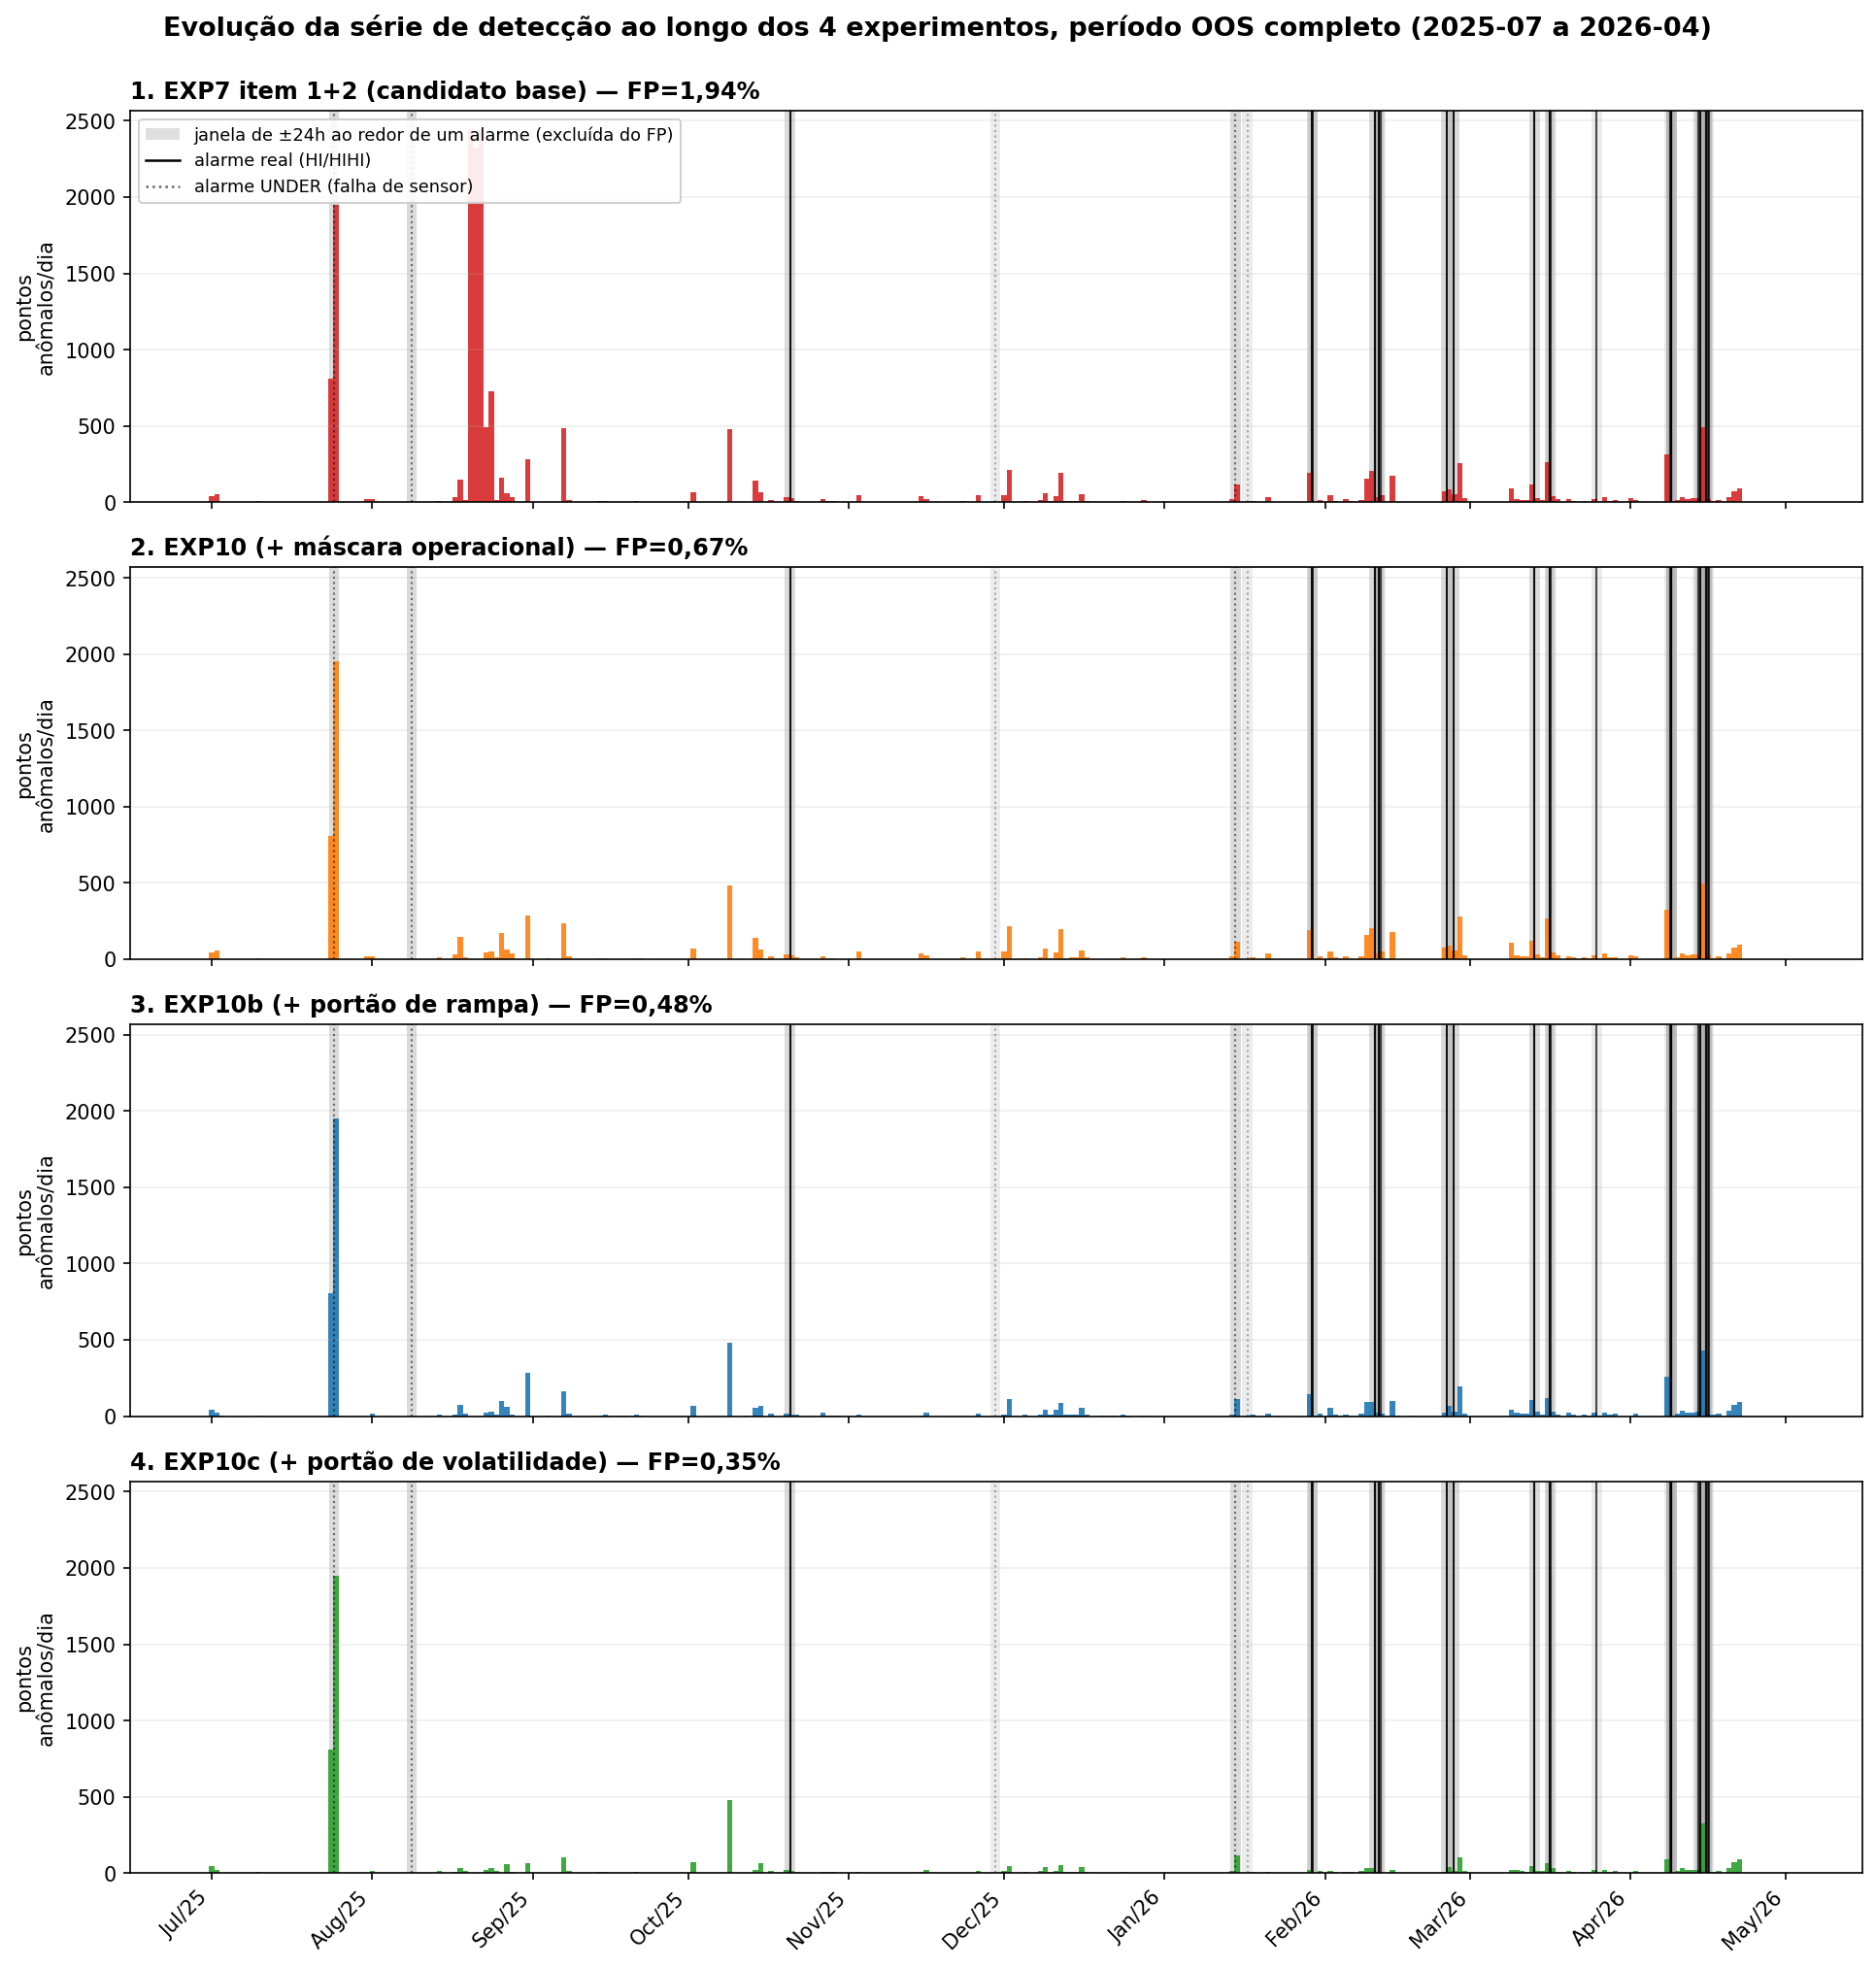
\includegraphics[width=\textwidth]{11_evolucao_4_experimentos.png}
\caption{Pontos anômalos por dia em cada um dos 4 experimentos, mesma
escala vertical. A linha 1 (EXP7) tem o bloco maciço de 20--22/08
(desligamento mal rotulado); a linha 2 (EXP10) já o elimina por
completo, confirmando que a correção age exatamente onde devia. Das
linhas 2 a 4, os picos residuais fora da faixa cinza (fim de agosto,
início de outubro, alguns dias em fevereiro/março/abril) encolhem
progressivamente -- efeito cumulativo do portão de rampa e depois do
portão de volatilidade. Os picos \emph{dentro} da faixa cinza (detecção
de alarme real) ficam idênticos nas 4 linhas, como esperado -- nenhuma
das correções toca a detecção.}
\label{fig:evolucao-4-experimentos}
\end{figure}

Em detalhe, comparando só a primeira e a última etapa lado a lado:

\begin{figure}[H]
\centering
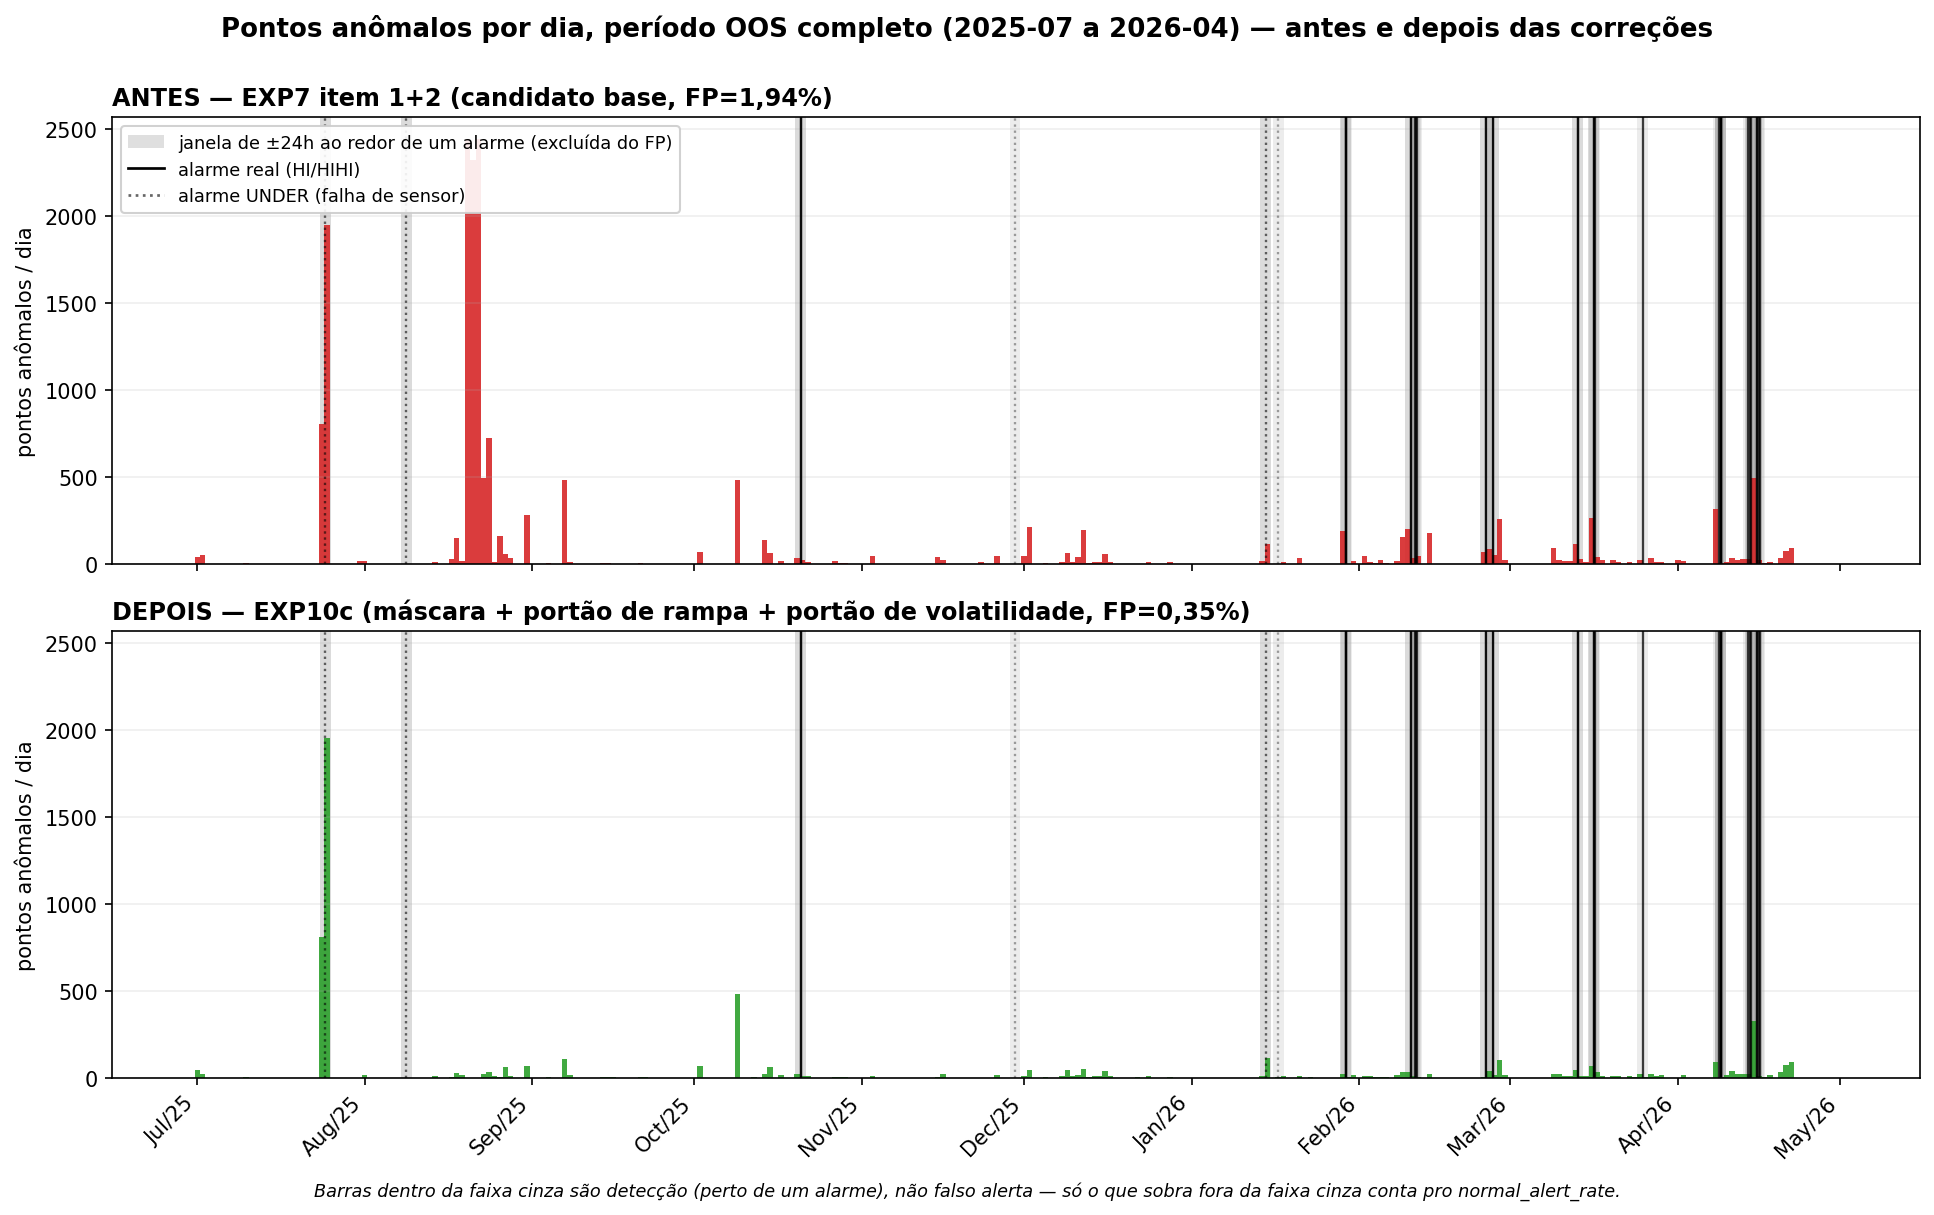
\includegraphics[width=\textwidth]{08_serie_completa_antes_depois.png}
\caption{Pontos anômalos por dia, período OOS completo, EXP7 item1+2 vs.
EXP10c (as três correções). Os picos dentro da faixa cinza (perto de um
alarme, sólida = HI/HIHI, pontilhada = UNDER) são detecção, não falso
alerta, e por isso ficam praticamente idênticos entre os painéis. O
bloco vermelho maciço de 20--22/08 (o desligamento mal rotulado)
desaparece completamente no painel de baixo, e os picos residuais fora
da faixa cinza (fim de agosto, início de outubro) ficam visivelmente
menores -- efeito combinado dos portões de rampa e de volatilidade.}
\label{fig:serie-completa}
\end{figure}

Dois pontos que a Figura~\ref{fig:serie-completa} deixa explícitos:

\begin{itemize}
  \item O pico isolado logo após ``Ago/25'' (na verdade 24--25/07) fica
        \textbf{idêntico} nos dois painéis porque cai dentro da janela de
        um alarme \texttt{UNDER} -- já não contava como falso alerta em
        nenhum dos dois candidatos, então não era esperado que mudasse.
        Serve de contraste: nem todo pico grande é falso alerta, e nem
        todo falso alerta é um pico pequeno.
  \item Os picos que ainda sobram \emph{fora} de qualquer faixa cinza no
        painel de baixo (poucos dias entre outubro e abril) são o
        resíduo de 0,35\% não endereçado por nenhuma das três correções
        -- majoritariamente falha de sensor pontual e correlação com
        outro alarme fora do escopo de 2 sensores (ver
        Seção~\ref{sec:proximos-passos}).
\end{itemize}

Um zoom no trecho de 15/08 a 10/09/2025 (que cobre o desligamento e a
maior parte das rampas de carga investigadas) deixa a comparação ainda
mais direta:

\begin{figure}[H]
\centering
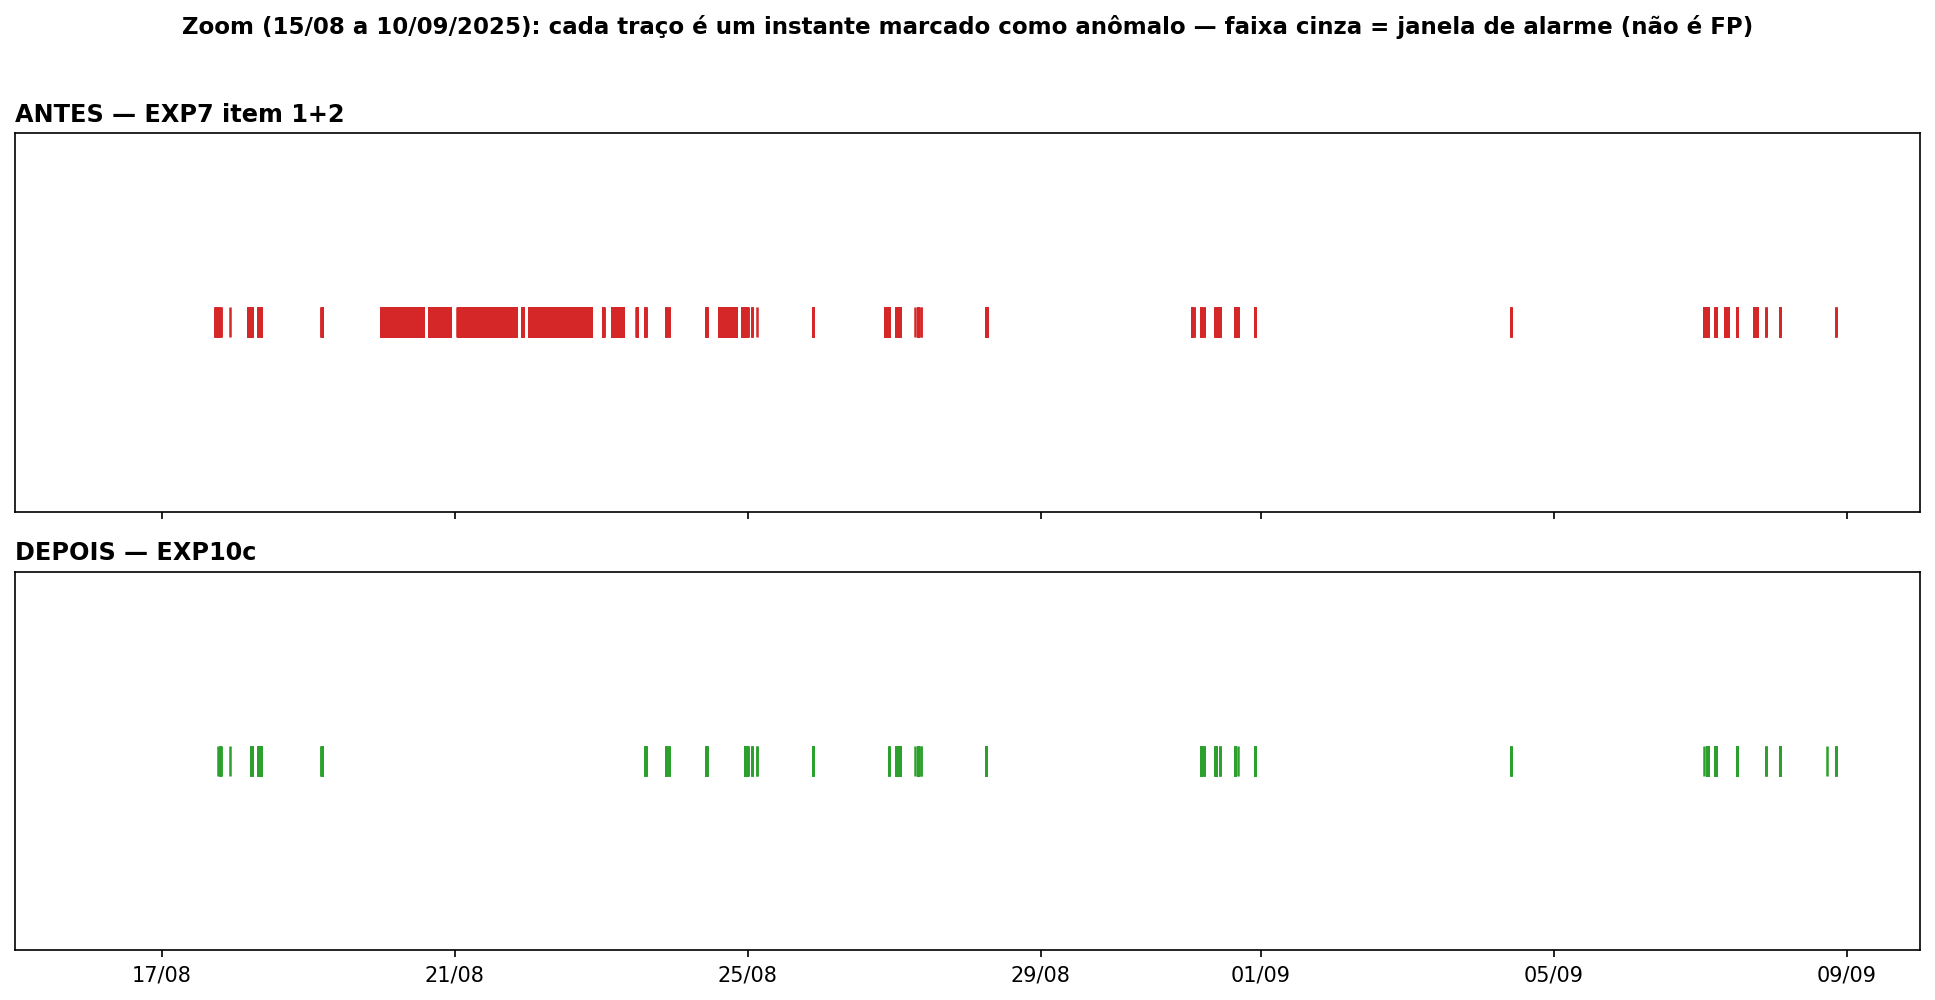
\includegraphics[width=\textwidth]{09_zoom_antes_depois.png}
\caption{Cada traço vertical é um instante de 30s marcado como anômalo,
EXP7 item1+2 vs. EXP10c. O bloco sólido de 19--23/08 (desligamento)
desaparece por completo; o traçado que sobra já é visivelmente mais
esparso que o intermediário do EXP10b (comparar com a versão anterior
deste relatório) -- efeito do portão de volatilidade sobre os episódios
de rampa que o portão de rampa sozinho não zerava totalmente.}
\end{figure}

\textbf{O novo candidato de referência} da série EXP5--EXP10:
\texttt{ocsvm} (percentil 99,9, debounce=1) sobre multiescala + textura
+ máscara operacional corrigida (\texttt{OFF\_TARGET\_ABS\_THRESHOLD}) +
portão de rampa (\texttt{ENABLE\_LOAD\_GATE}, janela curta) + portão de
volatilidade (\texttt{ENABLE\_VOLATILITY\_GATE}). Nenhuma das três
correções tocou no modelo de anomalia em si --- todas atuam inteiramente
na camada de pós-processamento/avaliação, sobre problemas de rotulagem e
de contexto operacional, não sobre o que o \texttt{ocsvm} aprendeu.

% =====================================================================
\section{O que ainda resta}
\label{sec:proximos-passos}
% =====================================================================

Os 0,35\% de falso alerta remanescente não têm mais um único bloco
dominante como no início -- o mapa de causas original (Seção~\ref{sec:metodo})
tinha duas fatias ainda não endereçadas por nenhuma das três correções:

\begin{itemize}
  \item \textbf{Contaminação por dropout de sensor} ($\sim$2,1\% do FP
        original): um dropout breve (\texttt{-40,x}) contamina a feature
        de tendência de 24h por até 24h depois, mesmo com o dado já
        normal de volta. Nenhuma das três correções deste relatório
        mira esse mecanismo especificamente.
  \item \textbf{Correlacionado com outro alarme real fora de escopo}
        ($\sim$9,7\%): picos que coincidem com alarmes de pressão/partida
        a gás (\texttt{PAL\_6240315}, \texttt{PI\_6240319\_AL}) do mesmo
        equipamento -- não é erro do modelo, é eco de um evento real que
        nossa avaliação de 2 sensores não credita. Resolver isso é uma
        decisão de metodologia de avaliação (ampliar a janela de exclusão
        pra outras categorias de alarme do catálogo), não um fix de
        modelo.
\end{itemize}

% =====================================================================
\section{O que foi inovador aqui}
% =====================================================================

\begin{itemize}
  \item \textbf{Método:} até este relatório, toda a série EXP5--EXP9
        avaliava candidatos pela métrica agregada
        (hit\_rate/normal\_alert\_rate) ou, no máximo, pelo breakdown
        preditivo/reativo/sem-detecção por alarme. Fragmentar a
        \emph{série de falso alerta} em episódios contínuos e investigar
        cada um contra dado bruto + catálogo completo é uma unidade de
        análise nova, que revelou estrutura (72,5\% em 10 episódios)
        onde a métrica agregada só mostrava um número.
  \item \textbf{Achado 1:} o falso alerta majoritário não era um
        problema do detector --- era um problema de rotulagem
        operacional que mascarava um evento real. A correção (segundo
        critério de off, independente, unido por OR) generaliza para
        qualquer grupo/sensor-alvo futuro sem precisar reajustar
        \texttt{RUNNING\_A}.
  \item \textbf{Achado 2:} reaproveitamos um mecanismo que já existia no
        código (portão de rampa) mas nunca tinha sido conectado ao
        pipeline que efetivamente usamos. A parte nova não foi a ideia
        --- foi (a) perceber que o padrão nos dados pedia exatamente essa
        ferramenta, e (b) descobrir, por simulação offline sistemática,
        que os parâmetros default do outro pipeline custavam detecção
        real, e recalibrar a janela de memória até o ponto de custo
        zero.
  \item \textbf{Achado 3:} a inovação real aqui não foi a primeira ideia
        (reaproveitar o portão de rampa pra vibração) --- foi
        \textbf{diagnosticar por que ela falhou} (taxa de variação não
        distingue rampa real de rampa de falha) e voltar pra evidência
        bruta (Figura~\ref{fig:rampa-exemplo}) pra perceber que o padrão
        físico certo era \emph{nível sustentado}, não \emph{taxa de
        subida} --- e só então escrever um mecanismo novo
        (\texttt{compute\_volatility\_index}) desenhado especificamente
        pra isso. Uma tentativa que não funciona, investigada até o fim,
        apontou o caminho certo em vez de ser só descartada.
  \item \textbf{Disciplina:} as três correções foram validadas por
        simulação offline \emph{antes} de qualquer submissão remota
        (reaproveitando o \texttt{is\_anom\_point} já cacheado em
        debounce=1), e por teste de fumaça sintético ponta-a-ponta antes
        do commit --- o mesmo padrão de rigor usado em toda a série
        EXP5--EXP9, aplicado agora à camada de pós-processamento. Nas
        três vezes, o resultado em produção bateu a simulação offline
        com menos de 0,01pp de diferença.
  \item \textbf{Resultado:} $-$82\% de falso alerta (1,94\%$\to$0,35\%)
        em quatro passos incrementais, custo zero de detecção em cada um
        deles, confirmado em produção (task remota) a cada etapa.
\end{itemize}

\end{document}
